\documentclass[11pt,a4paper]{article}
\usepackage[margin=2.2cm]{geometry}
\usepackage{amsmath,amssymb}
\usepackage{enumitem}
\usepackage{fancyhdr}
\usepackage{booktabs}
\usepackage{array}
\usepackage{graphicx}
\usepackage[most]{tcolorbox}
\usepackage{kotex}
\setmainhangulfont{Nanum Myeongjo}
\setsanshangulfont{Apple SD Gothic Neo}
\usepackage[hidelinks]{hyperref}

\pagestyle{fancy}
\fancyhf{}
\lhead{Datathon Statistics}
\rhead{pandas 흐름으로 따라가는 통계}
\cfoot{\thepage}
\setlength{\headheight}{14pt}
\setlength{\parindent}{0pt}
\setlength{\parskip}{0.45em}
\setlength{\emergencystretch}{2em}
\setlist[itemize]{leftmargin=1.3em,itemsep=0.2em,topsep=0.2em}
\setlist[enumerate]{leftmargin=1.6em,itemsep=0.2em,topsep=0.2em}
\renewcommand{\arraystretch}{1.15}
\AddToHook{cmd/section/before}{\clearpage}

\newcommand{\E}{\mathbb{E}}
\newcommand{\Var}{\operatorname{Var}}
\newcommand{\SD}{\mathrm{SD}}
\newcommand{\SE}{\mathrm{SE}}
\newcommand{\term}[1]{\textbf{#1}}
\newcommand{\code}[1]{\texttt{#1}}
\newcommand{\warn}{\textsf{\small 주의}\;}
% 강의노트 참조용 작은 주석
\newcommand{\nref}[1]{{\footnotesize\textsf{\color{blue!55!black}[Notes #1]}}}
\newcommand{\aside}[1]{{\footnotesize\color{black!65}#1}}
% 앞 장 내용을 보강/확장할 때 다는 주석, 뒤 장으로 넘기는 주석
\newcommand{\linkup}[1]{{\footnotesize\textsf{\color{green!40!black}[$\uparrow$ #1 보강]}}}
\newcommand{\fwd}[1]{{\footnotesize\textsf{\color{green!40!black}[$\to$ #1에서 자세히]}}}
\newcommand{\Ans}{\par\textbf{Answer.}\ }
\newcommand{\Just}{\par\textbf{Justification.}\ }

\newtcolorbox{codebox}{breakable,colback=black!3,colframe=black!45,boxrule=0.5pt,arc=1.5pt,
  left=4pt,right=4pt,top=2pt,bottom=2pt,fontupper=\small\ttfamily}
\newtcolorbox{hypbox}{breakable,colback=blue!3,colframe=blue!45!black,boxrule=0.6pt,arc=1.5pt,
  fonttitle=\bfseries\sffamily,title={추정 · 가설 · 검증}}
\newtcolorbox{keybox}[1]{breakable,colback=orange!4,colframe=orange!60!black,boxrule=0.6pt,arc=1.5pt,
  fonttitle=\bfseries\sffamily,title={#1}}

\begin{document}

\begin{center}
{\LARGE\textbf{pandas 흐름으로 따라가는 통계}}\\[0.4em]
{\large 추정 · 가설 · 검증 중심 정리 (\code{hiring\_practice.csv})}\\[0.3em]
{\small 각 장 = pandas 분석의 한 단계. 코드 $\to$ 실제 출력 $\to$ 개념 $\to$ 추정/가설/검증 순서로 읽습니다.\\
\nref{\dots} 는 Statistics 1 강의노트(\code{stats1-notes.pdf})의 해당 정의·정리 번호입니다.}
\end{center}

\vspace{0.5em}
\begin{center}\small
\begin{tabular}{@{}c l l l@{}}
\toprule
장 & pandas & 통계 개념 & 추정 / 가설 / 검증 \\
\midrule
1 & \code{read\_csv}, \code{info}, \code{isna} & 변수 종류, 결측, 측정오차, 편의 & 무엇을 추정할지 정하기 \\
2 & \code{describe} & 평균·중앙값·최빈값, SD, RMS, 자유도, 이탈값 & 중심과 퍼짐의 추정 \\
3 & \code{(x-x.mean())/x.std()} & 표준화, 정규근사, 백분위수 & 정규모형 가정 점검 \\
4 & \code{groupby().mean()} & 표본비율, SE, CLT & 점추정과 신뢰구간 \\
5 & \code{crosstab}, \code{scipy.stats} & $z$-test, $\chi^2$, $t$-test & 가설검정 \\
6 & \code{corr} & 산포도, 상관계수 & $r$ 추정, $\rho=0$ 검정 \\
7 & \code{smf.ols} & 회귀선, 평균의 그래프, 회귀효과 & 기울기 추정 \\
8 & \code{resid} & 잔차, RMSE, 잔차도 & 오차 추정, 기울기 검정 \\
\midrule
9 & \code{sample} (bootstrap) & 추정량의 성질 & bias, MSE, SE \\
10 & \code{mean}, \code{var} & 적률법(MoM), MLE & 추정량 만들기 \\
11 & -- & 가설 세우기, 검정력 & 검증 설계 \\
12 & \code{scipy.stats} & 검정 도구상자 13종 & 어떤 검정을 언제 \\
13 & \code{smf.ols} (다중) & 다중회귀 & 통제 후 효과의 추정·검증 \\
\bottomrule
\end{tabular}
\end{center}

\begin{keybox}{세 단어부터}
\begin{itemize}
\item \term{추정 (estimation)}: 모르는 모집단 값(parameter)을 데이터로 \emph{짐작}하는 것. 숫자 하나(\term{point estimate})와 그 불확실성(\term{SE}, \term{confidence interval})을 같이 냅니다.
\item \term{가설 (hypothesis)}: parameter에 대한 주장. ``차이 없음''을 $H_0$, 보이고 싶은 것을 $H_1$로 씁니다.
\item \term{검증 (testing)}: ``$H_0$가 맞다면 지금 데이터가 얼마나 이상한가''를 p-value로 재서 $H_0$를 기각할지 정합니다.
\end{itemize}
모든 장에서 이 세 가지를 반복합니다. 바뀌는 것은 \emph{무엇을} 추정하는가(평균, 비율, 상관, 기울기)뿐입니다.
\end{keybox}

\clearpage
\clearpage
% 세 책 공통: 앞쪽 "전체 흐름" 페이지. 각 책에서 % 세 책 공통: 앞쪽 "전체 흐름" 페이지. 각 책에서 % 세 책 공통: 앞쪽 "전체 흐름" 페이지. 각 책에서 \input{roadmap} 으로 넣는다.
\providecommand{\code}[1]{\texttt{#1}}
\newcolumntype{L}[1]{>{\raggedright\arraybackslash}p{#1}}
% 책별 장 표시 (작은 색 주석)
\newcommand{\Wc}[1]{{\scriptsize\textsf{\color{blue!60!black}[흐름 #1]}}}
\newcommand{\Hc}[1]{{\scriptsize\textsf{\color{orange!70!black}[응용 #1]}}}
\newcommand{\Ac}[1]{{\scriptsize\textsf{\color{green!45!black}[알고 #1]}}}
\newcommand{\Pc}[1]{{\scriptsize\textsf{\color{red!60!black}[실습 #1]}}}

\section*{먼저 읽기: 분석 전체 흐름과 책 안내}
\addcontentsline{toc}{section}{먼저 읽기: 분석 전체 흐름과 책 안내}

\textbf{네 권의 역할}
\begin{center}\small
\begin{tabular}{@{}l L{5.4cm} L{7.4cm}@{}}
\toprule
표시 & 책 (파일) & 역할 \\
\midrule
\Wc{} & pandas 흐름으로 따라가는 통계 (\code{pandas-stats-walkthrough}) & \textbf{기초}: 평균·SD·정규·상관·회귀·검정을 pandas 순서대로 \\
\Hc{} & 채용 데이터로 다시 배우는 통계 (\code{hiring-statistics-book}) & \textbf{응용}: 통제 회귀, logistic, Bayesian, 공정성으로 결론 내기 \\
\Ac{} & 알고리즘으로 보는 pandas (\code{algorithms-for-datathon}) & \textbf{도구}: 빠르고 정확한 코드, 결정트리·greedy 보조 분석 \\
\Pc{} & numpy·pandas로 직접 만드는 통계 (\code{stats-basics-workbook}) & \textbf{실습}: 빈칸 노트북으로 통계 공식을 직접 구현, 필요한 곳에 알고리즘 적용 \\
\bottomrule
\end{tabular}
\end{center}
\aside{※ 아래 표의 작은 색 주석이 ``이 단계는 어느 책 몇 장''입니다. 예: \Wc{5} = 흐름 책 5장, \Hc{6.9} = 응용 책 6.9절, \Ac{4} = 알고리즘 책 4장. 0장 = 응용 책 앞의 ``데이터 미리보기와 pandas 작동 원리''.}

\vspace{0.4em}
\textbf{Datathon 분석 흐름: 데이터를 받은 순간부터 발표까지}
\begin{center}\small
\renewcommand{\arraystretch}{1.25}
\begin{tabular}{@{}c L{3.3cm} L{4.6cm} L{5.6cm}@{}}
\toprule
단계 & 하는 일 & 대표 pandas 코드 & 해당 장 \\
\midrule
① & 질문을 통계 질문으로 & -- &
  \Hc{1} \Wc{1 추정·가설·검증 상자} \\
② & 불러오고 구조 확인 & \code{read\_csv}, \code{head}, \code{info} &
  \Hc{0.1–0.3} \Wc{1} \\
③ & 변수 분류 (결과 $Y$ / 보호속성 $A$ / 자격 $X$) & \code{dtypes}, \code{value\_counts} &
  \Hc{2} \Wc{1.1} \\
④ & 결측·이탈값 처리 & \code{isna}, \code{dropna}, \code{quantile} &
  \Hc{0.7, 2.4} \Wc{1.3, 2.3} \\
⑤ & 분포 요약 (중심, 퍼짐, 정규성) & \code{describe}, \code{std}, \code{(x-x.mean())/x.std()} &
  \Wc{2, 3} \Hc{3.1} \Ac{3 분위수} \Pc{1–3} \\
⑥ & 그룹별 합격률과 신뢰구간 & \code{groupby().mean()} &
  \Hc{0.5, 3.2} \Wc{4} \Ac{4 groupby 내부} \Pc{4} \\
⑦ & 교란 변수 확인 (Simpson) & \code{crosstab}, \code{groupby([a,b])} &
  \Hc{3.3} \Wc{12 ⑧} \\
⑧ & 가설검정 (차이가 우연인가) & \code{proportions\_ztest}, \code{chi2\_contingency}, \code{ttest\_ind} &
  \Wc{5, 11, 12} \Hc{5} \Pc{5–7} \\
⑨ & 상관과 단순회귀 & \code{corr}, \code{pd.cut}, \code{smf.ols} &
  \Wc{6–8} \Ac{5 pd.cut} \Pc{8–9} \\
⑩ & 통제 회귀와 interaction (핵심) & \code{smf.ols("y \~{} A + X")}, \code{A*B} &
  \Hc{0.8–0.9, 6} \Wc{13} \Pc{10} \\
⑪ & 다른 방법으로 재확인 & \code{smf.logit}, \code{rng.beta}, \code{DecisionTreeClassifier} &
  \Hc{7, 8} \Wc{9 bootstrap} \Pc{6, 11} \\
⑫ & 공정성 지표와 한계 & \code{rate["F"]/rate["M"]}, \code{idxmin} &
  \Hc{9} \Ac{8 minimax} \\
⑬ & 정리와 발표 & -- &
  \Hc{9.2 결론 문장, 11 체크리스트} \Wc{14 요약} \Ac{11} \\
\bottomrule
\end{tabular}
\end{center}
\aside{※ 이론이 막히면: 추정량·MoM·MLE \Wc{9–10} \Hc{4}, 가설 세우기·검정력 \Wc{11}, 코드가 느리면 \Ac{1–2, 4}. 한 번에 돌려 보기: \code{python3 algo\_toolkit.py hiring\_practice.csv} (⑥⑦⑨⑪⑫ 요약).}

\clearpage
\textbf{6시간 읽기 계획 (읽기 편한 순서)}
\begin{center}\small
\renewcommand{\arraystretch}{1.25}
\begin{tabular}{@{}l L{4.6cm} L{6.6cm} r@{}}
\toprule
시간 & 무엇을 & 어디를 & 분 \\
\midrule
0:00 & 데이터와 pandas 감 잡기 & \Hc{0} 전체, \Hc{1} 전체 지도 & 30 \\
0:30 & 기초 통계 1: 요약과 분포 & \Wc{1–3} (\code{describe}, 표준화, 정규근사) & 50 \\
1:20 & 기초 통계 2: 추정과 검정 & \Wc{4–5} (신뢰구간, $z$/$\chi^2$/$t$) & 40 \\
2:00 & \textit{휴식} & & 10 \\
2:10 & 기초 통계 3: 상관과 회귀 & \Wc{6–8} (회귀 효과, RMSE, 잔차도) & 50 \\
3:00 & 검정 고르는 법 & \Wc{12} 검정 도구상자 (표 + 관심 있는 카드만) & 30 \\
3:30 & 응용 1: 통제와 interaction & \Hc{3, 6} + 각 장 끝 ``pandas 코드'' 직접 실행 & 50 \\
4:20 & \textit{휴식} & & 10 \\
4:30 & 응용 2: 재확인 & \Hc{7} logistic, \Hc{8} Bayesian (8.4 ``왜''는 꼭) & 40 \\
5:10 & 결론과 한계 & \Hc{9}, \Hc{11} 체크리스트, \Ac{표지 결론표} & 20 \\
5:30 & 도구 실행과 발표 문장 연습 & \code{algo\_toolkit.py} 실행, \Hc{9.2} 문장을 내 말로 & 30 \\
(다음 날) & 코드로 손에 익히기 & \Pc{0–12} 빈칸 노트북 (\code{stats\_basics\_practice.ipynb}) & 120 \\
\bottomrule
\end{tabular}
\end{center}
\aside{※ 범위 밖 (학부 1–2학년 목표를 넘는 것): sklearn을 쓰는 \Ac{6–7}의 결정트리와 \code{advanced/} 폴더의 분류 워크북은 나중에 선택으로.}\\
\aside{※ 건너뛰어도 되는 곳 (나중에 참고용): \Wc{9–11, 13}, \Hc{4, 10}, \Ac{1–10} 본문, 모든 연습 문제. 시간이 남으면 \Wc{15} 연습 문제 1–8번부터.}\\
\aside{※ 각 장은 새 페이지에서 시작하고, 목차의 항목을 누르면 그 쪽으로 이동합니다.}
 으로 넣는다.
\providecommand{\code}[1]{\texttt{#1}}
\newcolumntype{L}[1]{>{\raggedright\arraybackslash}p{#1}}
% 책별 장 표시 (작은 색 주석)
\newcommand{\Wc}[1]{{\scriptsize\textsf{\color{blue!60!black}[흐름 #1]}}}
\newcommand{\Hc}[1]{{\scriptsize\textsf{\color{orange!70!black}[응용 #1]}}}
\newcommand{\Ac}[1]{{\scriptsize\textsf{\color{green!45!black}[알고 #1]}}}
\newcommand{\Pc}[1]{{\scriptsize\textsf{\color{red!60!black}[실습 #1]}}}

\section*{먼저 읽기: 분석 전체 흐름과 책 안내}
\addcontentsline{toc}{section}{먼저 읽기: 분석 전체 흐름과 책 안내}

\textbf{네 권의 역할}
\begin{center}\small
\begin{tabular}{@{}l L{5.4cm} L{7.4cm}@{}}
\toprule
표시 & 책 (파일) & 역할 \\
\midrule
\Wc{} & pandas 흐름으로 따라가는 통계 (\code{pandas-stats-walkthrough}) & \textbf{기초}: 평균·SD·정규·상관·회귀·검정을 pandas 순서대로 \\
\Hc{} & 채용 데이터로 다시 배우는 통계 (\code{hiring-statistics-book}) & \textbf{응용}: 통제 회귀, logistic, Bayesian, 공정성으로 결론 내기 \\
\Ac{} & 알고리즘으로 보는 pandas (\code{algorithms-for-datathon}) & \textbf{도구}: 빠르고 정확한 코드, 결정트리·greedy 보조 분석 \\
\Pc{} & numpy·pandas로 직접 만드는 통계 (\code{stats-basics-workbook}) & \textbf{실습}: 빈칸 노트북으로 통계 공식을 직접 구현, 필요한 곳에 알고리즘 적용 \\
\bottomrule
\end{tabular}
\end{center}
\aside{※ 아래 표의 작은 색 주석이 ``이 단계는 어느 책 몇 장''입니다. 예: \Wc{5} = 흐름 책 5장, \Hc{6.9} = 응용 책 6.9절, \Ac{4} = 알고리즘 책 4장. 0장 = 응용 책 앞의 ``데이터 미리보기와 pandas 작동 원리''.}

\vspace{0.4em}
\textbf{Datathon 분석 흐름: 데이터를 받은 순간부터 발표까지}
\begin{center}\small
\renewcommand{\arraystretch}{1.25}
\begin{tabular}{@{}c L{3.3cm} L{4.6cm} L{5.6cm}@{}}
\toprule
단계 & 하는 일 & 대표 pandas 코드 & 해당 장 \\
\midrule
① & 질문을 통계 질문으로 & -- &
  \Hc{1} \Wc{1 추정·가설·검증 상자} \\
② & 불러오고 구조 확인 & \code{read\_csv}, \code{head}, \code{info} &
  \Hc{0.1–0.3} \Wc{1} \\
③ & 변수 분류 (결과 $Y$ / 보호속성 $A$ / 자격 $X$) & \code{dtypes}, \code{value\_counts} &
  \Hc{2} \Wc{1.1} \\
④ & 결측·이탈값 처리 & \code{isna}, \code{dropna}, \code{quantile} &
  \Hc{0.7, 2.4} \Wc{1.3, 2.3} \\
⑤ & 분포 요약 (중심, 퍼짐, 정규성) & \code{describe}, \code{std}, \code{(x-x.mean())/x.std()} &
  \Wc{2, 3} \Hc{3.1} \Ac{3 분위수} \Pc{1–3} \\
⑥ & 그룹별 합격률과 신뢰구간 & \code{groupby().mean()} &
  \Hc{0.5, 3.2} \Wc{4} \Ac{4 groupby 내부} \Pc{4} \\
⑦ & 교란 변수 확인 (Simpson) & \code{crosstab}, \code{groupby([a,b])} &
  \Hc{3.3} \Wc{12 ⑧} \\
⑧ & 가설검정 (차이가 우연인가) & \code{proportions\_ztest}, \code{chi2\_contingency}, \code{ttest\_ind} &
  \Wc{5, 11, 12} \Hc{5} \Pc{5–7} \\
⑨ & 상관과 단순회귀 & \code{corr}, \code{pd.cut}, \code{smf.ols} &
  \Wc{6–8} \Ac{5 pd.cut} \Pc{8–9} \\
⑩ & 통제 회귀와 interaction (핵심) & \code{smf.ols("y \~{} A + X")}, \code{A*B} &
  \Hc{0.8–0.9, 6} \Wc{13} \Pc{10} \\
⑪ & 다른 방법으로 재확인 & \code{smf.logit}, \code{rng.beta}, \code{DecisionTreeClassifier} &
  \Hc{7, 8} \Wc{9 bootstrap} \Pc{6, 11} \\
⑫ & 공정성 지표와 한계 & \code{rate["F"]/rate["M"]}, \code{idxmin} &
  \Hc{9} \Ac{8 minimax} \\
⑬ & 정리와 발표 & -- &
  \Hc{9.2 결론 문장, 11 체크리스트} \Wc{14 요약} \Ac{11} \\
\bottomrule
\end{tabular}
\end{center}
\aside{※ 이론이 막히면: 추정량·MoM·MLE \Wc{9–10} \Hc{4}, 가설 세우기·검정력 \Wc{11}, 코드가 느리면 \Ac{1–2, 4}. 한 번에 돌려 보기: \code{python3 algo\_toolkit.py hiring\_practice.csv} (⑥⑦⑨⑪⑫ 요약).}

\clearpage
\textbf{6시간 읽기 계획 (읽기 편한 순서)}
\begin{center}\small
\renewcommand{\arraystretch}{1.25}
\begin{tabular}{@{}l L{4.6cm} L{6.6cm} r@{}}
\toprule
시간 & 무엇을 & 어디를 & 분 \\
\midrule
0:00 & 데이터와 pandas 감 잡기 & \Hc{0} 전체, \Hc{1} 전체 지도 & 30 \\
0:30 & 기초 통계 1: 요약과 분포 & \Wc{1–3} (\code{describe}, 표준화, 정규근사) & 50 \\
1:20 & 기초 통계 2: 추정과 검정 & \Wc{4–5} (신뢰구간, $z$/$\chi^2$/$t$) & 40 \\
2:00 & \textit{휴식} & & 10 \\
2:10 & 기초 통계 3: 상관과 회귀 & \Wc{6–8} (회귀 효과, RMSE, 잔차도) & 50 \\
3:00 & 검정 고르는 법 & \Wc{12} 검정 도구상자 (표 + 관심 있는 카드만) & 30 \\
3:30 & 응용 1: 통제와 interaction & \Hc{3, 6} + 각 장 끝 ``pandas 코드'' 직접 실행 & 50 \\
4:20 & \textit{휴식} & & 10 \\
4:30 & 응용 2: 재확인 & \Hc{7} logistic, \Hc{8} Bayesian (8.4 ``왜''는 꼭) & 40 \\
5:10 & 결론과 한계 & \Hc{9}, \Hc{11} 체크리스트, \Ac{표지 결론표} & 20 \\
5:30 & 도구 실행과 발표 문장 연습 & \code{algo\_toolkit.py} 실행, \Hc{9.2} 문장을 내 말로 & 30 \\
(다음 날) & 코드로 손에 익히기 & \Pc{0–12} 빈칸 노트북 (\code{stats\_basics\_practice.ipynb}) & 120 \\
\bottomrule
\end{tabular}
\end{center}
\aside{※ 범위 밖 (학부 1–2학년 목표를 넘는 것): sklearn을 쓰는 \Ac{6–7}의 결정트리와 \code{advanced/} 폴더의 분류 워크북은 나중에 선택으로.}\\
\aside{※ 건너뛰어도 되는 곳 (나중에 참고용): \Wc{9–11, 13}, \Hc{4, 10}, \Ac{1–10} 본문, 모든 연습 문제. 시간이 남으면 \Wc{15} 연습 문제 1–8번부터.}\\
\aside{※ 각 장은 새 페이지에서 시작하고, 목차의 항목을 누르면 그 쪽으로 이동합니다.}
 으로 넣는다.
\providecommand{\code}[1]{\texttt{#1}}
\newcolumntype{L}[1]{>{\raggedright\arraybackslash}p{#1}}
% 책별 장 표시 (작은 색 주석)
\newcommand{\Wc}[1]{{\scriptsize\textsf{\color{blue!60!black}[흐름 #1]}}}
\newcommand{\Hc}[1]{{\scriptsize\textsf{\color{orange!70!black}[응용 #1]}}}
\newcommand{\Ac}[1]{{\scriptsize\textsf{\color{green!45!black}[알고 #1]}}}
\newcommand{\Pc}[1]{{\scriptsize\textsf{\color{red!60!black}[실습 #1]}}}

\section*{먼저 읽기: 분석 전체 흐름과 책 안내}
\addcontentsline{toc}{section}{먼저 읽기: 분석 전체 흐름과 책 안내}

\textbf{네 권의 역할}
\begin{center}\small
\begin{tabular}{@{}l L{5.4cm} L{7.4cm}@{}}
\toprule
표시 & 책 (파일) & 역할 \\
\midrule
\Wc{} & pandas 흐름으로 따라가는 통계 (\code{pandas-stats-walkthrough}) & \textbf{기초}: 평균·SD·정규·상관·회귀·검정을 pandas 순서대로 \\
\Hc{} & 채용 데이터로 다시 배우는 통계 (\code{hiring-statistics-book}) & \textbf{응용}: 통제 회귀, logistic, Bayesian, 공정성으로 결론 내기 \\
\Ac{} & 알고리즘으로 보는 pandas (\code{algorithms-for-datathon}) & \textbf{도구}: 빠르고 정확한 코드, 결정트리·greedy 보조 분석 \\
\Pc{} & numpy·pandas로 직접 만드는 통계 (\code{stats-basics-workbook}) & \textbf{실습}: 빈칸 노트북으로 통계 공식을 직접 구현, 필요한 곳에 알고리즘 적용 \\
\bottomrule
\end{tabular}
\end{center}
\aside{※ 아래 표의 작은 색 주석이 ``이 단계는 어느 책 몇 장''입니다. 예: \Wc{5} = 흐름 책 5장, \Hc{6.9} = 응용 책 6.9절, \Ac{4} = 알고리즘 책 4장. 0장 = 응용 책 앞의 ``데이터 미리보기와 pandas 작동 원리''.}

\vspace{0.4em}
\textbf{Datathon 분석 흐름: 데이터를 받은 순간부터 발표까지}
\begin{center}\small
\renewcommand{\arraystretch}{1.25}
\begin{tabular}{@{}c L{3.3cm} L{4.6cm} L{5.6cm}@{}}
\toprule
단계 & 하는 일 & 대표 pandas 코드 & 해당 장 \\
\midrule
① & 질문을 통계 질문으로 & -- &
  \Hc{1} \Wc{1 추정·가설·검증 상자} \\
② & 불러오고 구조 확인 & \code{read\_csv}, \code{head}, \code{info} &
  \Hc{0.1–0.3} \Wc{1} \\
③ & 변수 분류 (결과 $Y$ / 보호속성 $A$ / 자격 $X$) & \code{dtypes}, \code{value\_counts} &
  \Hc{2} \Wc{1.1} \\
④ & 결측·이탈값 처리 & \code{isna}, \code{dropna}, \code{quantile} &
  \Hc{0.7, 2.4} \Wc{1.3, 2.3} \\
⑤ & 분포 요약 (중심, 퍼짐, 정규성) & \code{describe}, \code{std}, \code{(x-x.mean())/x.std()} &
  \Wc{2, 3} \Hc{3.1} \Ac{3 분위수} \Pc{1–3} \\
⑥ & 그룹별 합격률과 신뢰구간 & \code{groupby().mean()} &
  \Hc{0.5, 3.2} \Wc{4} \Ac{4 groupby 내부} \Pc{4} \\
⑦ & 교란 변수 확인 (Simpson) & \code{crosstab}, \code{groupby([a,b])} &
  \Hc{3.3} \Wc{12 ⑧} \\
⑧ & 가설검정 (차이가 우연인가) & \code{proportions\_ztest}, \code{chi2\_contingency}, \code{ttest\_ind} &
  \Wc{5, 11, 12} \Hc{5} \Pc{5–7} \\
⑨ & 상관과 단순회귀 & \code{corr}, \code{pd.cut}, \code{smf.ols} &
  \Wc{6–8} \Ac{5 pd.cut} \Pc{8–9} \\
⑩ & 통제 회귀와 interaction (핵심) & \code{smf.ols("y \~{} A + X")}, \code{A*B} &
  \Hc{0.8–0.9, 6} \Wc{13} \Pc{10} \\
⑪ & 다른 방법으로 재확인 & \code{smf.logit}, \code{rng.beta}, \code{DecisionTreeClassifier} &
  \Hc{7, 8} \Wc{9 bootstrap} \Pc{6, 11} \\
⑫ & 공정성 지표와 한계 & \code{rate["F"]/rate["M"]}, \code{idxmin} &
  \Hc{9} \Ac{8 minimax} \\
⑬ & 정리와 발표 & -- &
  \Hc{9.2 결론 문장, 11 체크리스트} \Wc{14 요약} \Ac{11} \\
\bottomrule
\end{tabular}
\end{center}
\aside{※ 이론이 막히면: 추정량·MoM·MLE \Wc{9–10} \Hc{4}, 가설 세우기·검정력 \Wc{11}, 코드가 느리면 \Ac{1–2, 4}. 한 번에 돌려 보기: \code{python3 algo\_toolkit.py hiring\_practice.csv} (⑥⑦⑨⑪⑫ 요약).}

\clearpage
\textbf{6시간 읽기 계획 (읽기 편한 순서)}
\begin{center}\small
\renewcommand{\arraystretch}{1.25}
\begin{tabular}{@{}l L{4.6cm} L{6.6cm} r@{}}
\toprule
시간 & 무엇을 & 어디를 & 분 \\
\midrule
0:00 & 데이터와 pandas 감 잡기 & \Hc{0} 전체, \Hc{1} 전체 지도 & 30 \\
0:30 & 기초 통계 1: 요약과 분포 & \Wc{1–3} (\code{describe}, 표준화, 정규근사) & 50 \\
1:20 & 기초 통계 2: 추정과 검정 & \Wc{4–5} (신뢰구간, $z$/$\chi^2$/$t$) & 40 \\
2:00 & \textit{휴식} & & 10 \\
2:10 & 기초 통계 3: 상관과 회귀 & \Wc{6–8} (회귀 효과, RMSE, 잔차도) & 50 \\
3:00 & 검정 고르는 법 & \Wc{12} 검정 도구상자 (표 + 관심 있는 카드만) & 30 \\
3:30 & 응용 1: 통제와 interaction & \Hc{3, 6} + 각 장 끝 ``pandas 코드'' 직접 실행 & 50 \\
4:20 & \textit{휴식} & & 10 \\
4:30 & 응용 2: 재확인 & \Hc{7} logistic, \Hc{8} Bayesian (8.4 ``왜''는 꼭) & 40 \\
5:10 & 결론과 한계 & \Hc{9}, \Hc{11} 체크리스트, \Ac{표지 결론표} & 20 \\
5:30 & 도구 실행과 발표 문장 연습 & \code{algo\_toolkit.py} 실행, \Hc{9.2} 문장을 내 말로 & 30 \\
(다음 날) & 코드로 손에 익히기 & \Pc{0–12} 빈칸 노트북 (\code{stats\_basics\_practice.ipynb}) & 120 \\
\bottomrule
\end{tabular}
\end{center}
\aside{※ 범위 밖 (학부 1–2학년 목표를 넘는 것): sklearn을 쓰는 \Ac{6–7}의 결정트리와 \code{advanced/} 폴더의 분류 워크북은 나중에 선택으로.}\\
\aside{※ 건너뛰어도 되는 곳 (나중에 참고용): \Wc{9–11, 13}, \Hc{4, 10}, \Ac{1–10} 본문, 모든 연습 문제. 시간이 남으면 \Wc{15} 연습 문제 1–8번부터.}\\
\aside{※ 각 장은 새 페이지에서 시작하고, 목차의 항목을 누르면 그 쪽으로 이동합니다.}

\clearpage
\renewcommand{\contentsname}{목차 (Contents)}
\tableofcontents

%=================================================
\section{불러오기와 구조 파악}

\begin{codebox}
df = pd.read\_csv("hiring\_practice.csv")\\
df.shape \hfill \# (600, 7)\\
df.dtypes; df.isna().sum() \hfill \# test\_score만 결측 18개
\end{codebox}

\subsection{변수의 종류}
\begin{center}
\begin{tabular}{@{}l l l@{}}
\toprule
열 & 종류 & 쓸 수 있는 요약 \\
\midrule
\code{gender}, \code{hired} & binary (0/1) & 비율 \\
\code{department} & nominal (순서 없는 범주) & 빈도, 최빈값 \\
\code{degree} & ordinal (순서 있는 범주) & 빈도, 최빈값, 중앙값 \\
\code{years\_experience} & discrete (정수) & 평균, 중앙값, SD \\
\code{test\_score} & continuous & 평균, 중앙값, SD, 분포 \\
\code{applicant\_id} & identifier & 쓰지 않음 \\
\bottomrule
\end{tabular}
\end{center}
\aside{※ 종류가 곧 방법을 정합니다. 평균은 수량에만, 비율은 범주에만 의미가 있습니다.}

\subsection{데이터 = 확률변수의 실현값}
강의노트의 출발점: 데이터 $x_1,\dots,x_n$은 확률변수 $X_1,\dots,X_n$의 \term{realization}이고, 보통 \term{IID} (독립, 같은 분포)라고 가정합니다. \nref{§1.4}\\
\aside{※ 그래서 ``표본에서 계산한 값''은 표본이 바뀌면 달라지는 \emph{확률변수}이고, 이 흔들림을 재는 것이 추정·검증의 핵심입니다.}

\subsection{측정오차와 편의}
\begin{itemize}
\item \term{측정오차 (measurement error)}: 관측값 $=$ 참값 $+$ 오차. \code{test\_score}는 ``실력''을 시험 한 번으로 잰 값이라 우연 오차가 섞여 있습니다.\\
\aside{※ 우연 오차는 평균에서는 상쇄되지만 SD는 키우고, 다른 변수와의 상관 $r$과 회귀 기울기를 0 쪽으로 줄입니다 (\term{attenuation}).}
\item \term{편의 (bias)}: 우연이 아니라 \emph{한쪽으로 일관되게} 틀리는 것. 두 가지 의미로 쓰입니다.
  \begin{itemize}
  \item 자료의 편의: 채점 기준이 한 집단에 불리하거나, 특정 집단만 지원하는 경우 (\term{selection bias}). 표본을 늘려도 사라지지 않습니다.
  \item 추정량의 편의: $\text{bias}(T)=\E[T]-\theta$. \nref{Def 7.2} 2장의 $n-1$이 여기서 나옵니다. \fwd{9장}
  \end{itemize}
\item \term{결측 (missing)}: 18행 (3\%). 결측 18명 중 합격자 4명으로 전체 합격률과 비슷하므로 \code{dropna()}로 제외해도 큰 편의는 없다고 판단합니다.
\end{itemize}

\begin{hypbox}
여기서는 아직 계산하지 않고 \textbf{무엇을 추정·검증할지}를 정합니다.
\begin{itemize}
\item 추정 대상: 성별 합격 확률 $p_M,p_F$, 그 차이 $p_M-p_F$, 점수가 합격에 주는 효과(기울기).
\item 가설: $H_0: p_M=p_F$ (성별과 합격은 무관), $H_0$: 점수 평균은 성별로 같다.
\end{itemize}
\end{hypbox}

%=================================================
\section{describe(): 중심과 퍼짐}

\begin{codebox}
df[["years\_experience","test\_score","hired"]].describe()
\end{codebox}
\begin{center}
\begin{tabular}{@{}l r r r@{}}
\toprule
 & years\_experience & test\_score & hired \\
\midrule
count & 600 & 582 & 600 \\
mean & 4.455 & 65.235 & 0.322 \\
std & 1.962 & 11.657 & 0.468 \\
min & 0 & 29 & 0 \\
25\% & 3 & 58 & 0 \\
50\% & 4 & 65 & 0 \\
75\% & 6 & 73 & 1 \\
max & 11 & 100 & 1 \\
\bottomrule
\end{tabular}
\end{center}
\aside{※ \code{hired}의 mean 0.322 = 합격률 32.2\%. 0/1 변수의 평균은 비율입니다.}

\subsection{중심: 평균, 중앙값, 최빈값}
\begin{itemize}
\item \term{Mean} $\bar x=\frac1n\sum x_i$ \nref{Def 2.3}
\item \term{Median}: 정렬했을 때 가운데 값 (\term{order statistics} $x_{(1)}\le\dots\le x_{(n)}$의 가운데) \nref{Def 2.1, 2.4}
\item \term{Mode}: 가장 자주 나오는 값. \code{df.col.mode()}
\end{itemize}

\begin{center}
\begin{tabular}{@{}l c c c@{}}
\toprule
 & 평균 & 중앙값 & 최빈값 \\
\midrule
\code{test\_score} & 65.2 & 65 & 60 \\
\code{years\_experience} & 4.46 & 4 & 4 \\
\code{degree} & -- & (Bachelor) & Bachelor \\
\bottomrule
\end{tabular}
\end{center}

\begin{keybox}{언제 무엇을 쓰나}
\begin{center}
\begin{tabular}{@{}p{2cm} p{6cm} p{6cm}@{}}
\toprule
 & 장점 & 이럴 때 \\
\midrule
평균 & 모든 값을 사용, 합치기 쉬움 (두 집단 평균 $\to$ 전체 평균) & 대칭 분포, 이후 $t$-test·회귀에 쓸 때 \\
중앙값 & 극단값에 둔감 (\term{robust}) & 소득, 집값처럼 한쪽으로 긴 분포, 이탈값이 있을 때 \\
최빈값 & 범주형에도 정의됨 & nominal 변수, ``가장 흔한 유형'' \\
\bottomrule
\end{tabular}
\end{center}
\aside{※ 노트의 예: $(3,1,5,9,0,-1)$에서 $-1$을 $-1000$으로 바꾸면 평균은 $2.83\to-163.7$, 중앙값은 2 그대로. \nref{§2.2}}\\
\aside{※ 손실함수로 보면: 평균은 $\sum(x_i-c)^2$, 중앙값은 $\sum|x_i-c|$, 최빈값은 ``틀린 개수''를 최소화하는 $c$입니다 (문제지 주제).}\\
\aside{※ 평균 $\approx$ 중앙값이면 대칭, 평균 $>$ 중앙값이면 오른쪽 꼬리. \code{test\_score}는 65.2 vs 65로 거의 대칭, 경력은 4.46 vs 4로 약간 오른쪽 꼬리 (skewness 0.29).}
\end{keybox}

\subsection{퍼짐: 편차, RMS, 표준편차}
\textbf{1단계: 편차} $d_i=x_i-\bar x$. 평균에서 얼마나 떨어졌나. 그런데 $\sum d_i=0$이라 그냥 평균내면 항상 0입니다.

\textbf{2단계: RMS (제곱근-평균-제곱, root-mean-square).} 부호를 없애는 표준 방법:
\[
\text{RMS}(a_1,\dots,a_n)=\sqrt{\frac1n\sum a_i^2}\qquad(\text{제곱} \to \text{평균} \to \text{제곱근, 오른쪽부터 읽기}).
\]
\aside{※ RMS는 ``전형적인 크기''입니다. 예: $0,5,-8,7,-3$의 RMS $=\sqrt{147/5}\approx5.4$.}

\textbf{3단계: 표준편차 = 편차의 RMS.}
\[
\SD=\text{RMS}(d_1,\dots,d_n)=\sqrt{\frac1n\sum(x_i-\bar x)^2}.
\]
뜻: ``각 값이 평균에서 \emph{전형적으로} 얼마나 떨어져 있나''. \code{test\_score}의 SD $\approx11.6$점.

\textbf{4단계: 표본분산과 자유도.} 노트와 pandas의 기본값은 $n$ 대신 $n-1$로 나눕니다. \nref{Def 2.5}
\[
s^2=\frac1{n-1}\sum(x_i-\bar x)^2,\qquad s=\sqrt{s^2}.
\]
\begin{center}
\begin{tabular}{@{}l l r@{}}
\toprule
pandas & 분모 & \code{test\_score} \\
\midrule
\code{s.std(ddof=0)} & $n$ (= 편차의 RMS) & 11.647 \\
\code{s.std()} (기본, \code{ddof=1}) & $n-1$ & 11.657 \\
\bottomrule
\end{tabular}
\end{center}
\aside{※ numpy \code{np.std}는 기본이 \code{ddof=0}, pandas는 \code{ddof=1}. 결과가 미세하게 다르면 이 때문입니다.}

\begin{keybox}{왜 $n-1$인가: 자유도와 편의}
\begin{itemize}
\item \term{자유도 (degrees of freedom)}: 편차 $d_1,\dots,d_n$은 $\sum d_i=0$이라는 제약이 하나 있어서, $n-1$개를 정하면 마지막 하나는 자동으로 정해집니다. ``자유롭게 움직이는 값''이 $n-1$개.
\item 그래서 $n$으로 나누면 분산을 \emph{체계적으로 작게} 추정합니다: $\E\big[\frac1n\sum(X_i-\bar X)^2\big]=\frac{n-1}n\sigma^2$ (편의 있음). $n-1$로 나누면 $\E[S^2]=\sigma^2$ (\term{unbiased}). \nref{Def 7.2}
\item 정규분포에서는 $\frac{(n-1)S^2}{\sigma^2}\sim\chi^2(n-1)$. 자유도 $n-1$이 분포 이름에 그대로 들어갑니다. \nref{Thm 8.12}
\item 같은 원리로 회귀에서는 $\alpha,\beta$ 두 개를 추정하므로 잔차의 자유도가 $n-2$입니다 (8장). \nref{Prop 11.13}
\end{itemize}
\aside{※ $n=582$에서는 11.647 vs 11.657로 차이가 무시할 만합니다. $n$이 작을 때만 중요합니다.}
\end{keybox}

\subsection{사분위수, IQR, 이탈값}
\begin{itemize}
\item \term{Quantile}: $p$-분위수 = 자료의 $100p\%$가 그 아래에 있는 값. \nref{Def 2.7}
\item \term{Quartiles} $Q_1,Q_2,Q_3$ = 25, 50, 75\% 분위수. \term{IQR} $=Q_3-Q_1$ (가운데 50\%의 폭). \nref{Def 2.9}
\item \term{이탈값 (outlier)} 규칙 (boxplot의 수염): $[Q_1-1.5\,\text{IQR},\ Q_3+1.5\,\text{IQR}]$ 밖.
\end{itemize}
\begin{codebox}
q1, q3 = s.quantile([.25, .75]); iqr = q3 - q1 \hfill \# 58, 73, 15\\
s[(s < q1-1.5*iqr) | (s > q3+1.5*iqr)] \hfill \# 울타리 35.5, 95.5
\end{codebox}
결과: 29, 32, 33, 34, 35, 35, 35 (아래), 98, 100, 100 (위) — 10명. 경력은 11년 한 명.

\begin{center}
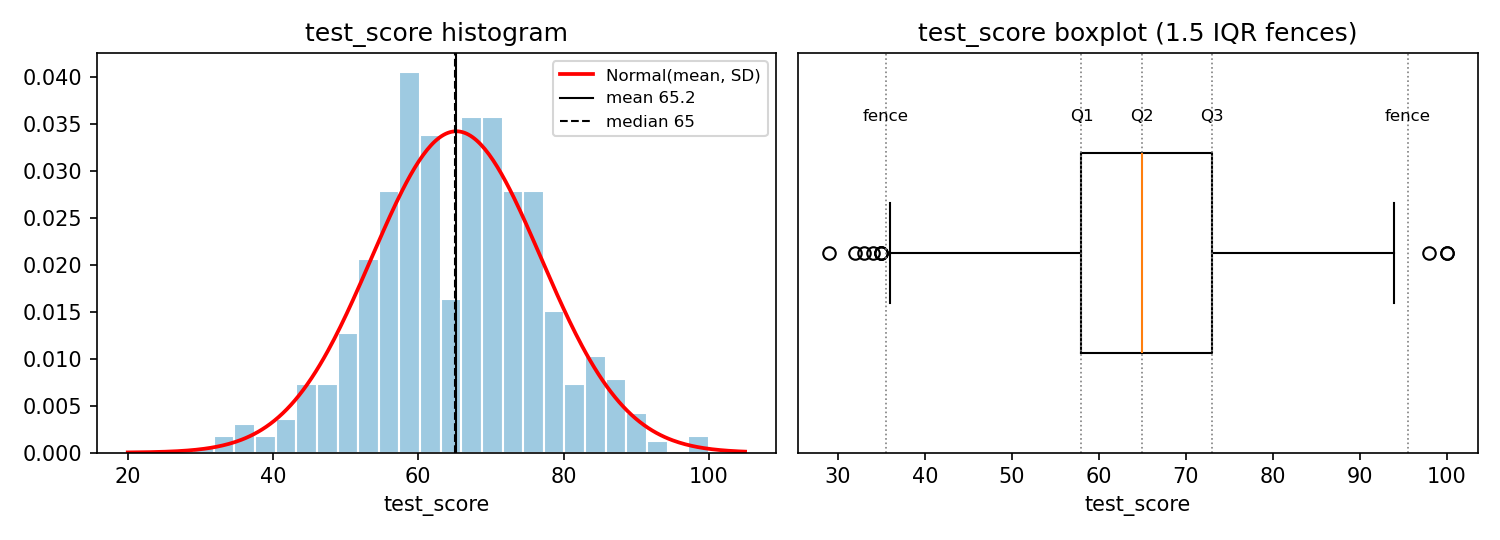
\includegraphics[width=\linewidth]{fig/dist.png}
\end{center}

\begin{keybox}{이탈값을 만나면}
\begin{enumerate}
\item \textbf{먼저 오류인지 확인} (입력 실수, 단위 실수). 오류면 고치거나 제거.
\item \textbf{진짜 값이면 지우지 않는다.} 100점은 가능한 점수입니다. 대신 이탈값을 빼고도 결론이 같은지 확인 (\term{sensitivity check}).
\item 영향 비교: 평균·SD·상관·회귀는 이탈값에 민감, 중앙값·IQR은 둔감.
\end{enumerate}
\aside{※ 노트 Anscombe's quartet의 3번 자료: 한 점 때문에 회귀선이 크게 틀어짐. \nref{Ex 11.15}}
\end{keybox}

\begin{hypbox}
\begin{itemize}
\item \textbf{추정}: 모집단 평균 $\mu$의 추정량 $\bar X$ (65.24), 모집단 SD $\sigma$의 추정량 $S$ (11.66).
\item \textbf{추정량 평가}: $\text{MSE}=\Var+\text{bias}^2$. \nref{Prop 7.4} $\bar X$는 unbiased이고 $\Var(\bar X)=\sigma^2/n$이므로 MSE $=\sigma^2/n$. \nref{Ex 7.5}
\item \textbf{SE}: $\SE(\bar X)=s/\sqrt n=11.66/\sqrt{582}=0.48$점. ``평균 65.2점은 $\pm$0.5점 정도 흔들린다.''
\end{itemize}
\end{hypbox}

%=================================================
\section{표준화와 정규근사}

\subsection{단위 변환과 표준점수}
\begin{codebox}
z = (s - s.mean()) / s.std()
\end{codebox}
\term{Standard units (z-score)}: $z=\dfrac{x-\bar x}{\SD}$ = ``평균보다 SD 몇 개만큼 위/아래인가''.
\begin{itemize}
\item 85점: $z=(85-65.24)/11.66=1.70$. 평균보다 1.7 SD 위.
\item 단위 변환 $y=ax+b$의 효과: 평균 $\to a\bar x+b$, SD $\to|a|\,\SD$ (더하기는 SD에 영향 없음). \nref{Lemma 8.6}\\
\aside{※ 점수를 10으로 나누면 평균 6.52, SD 1.17. 하지만 $z$-score는 그대로입니다. 그래서 $z$는 단위와 무관한 비교 척도이고, 상관계수(6장)도 같은 이유로 단위와 무관합니다.}
\item $X\sim N(\mu,\sigma^2)\iff Z=(X-\mu)/\sigma\sim N(0,1)$. \nref{Cor 8.7}
\end{itemize}

\subsection{정규분포곡선과 표준정규곡선 아래의 면적}
표준정규곡선 $\phi(z)=\frac1{\sqrt{2\pi}}e^{-z^2/2}$는 0에서 대칭인 종 모양이고, 전체 면적은 1입니다. \textbf{면적 = 확률 = 비율.}
\begin{center}
\begin{tabular}{@{}l l l@{}}
\toprule
구하는 것 & 식 & Python (\code{from scipy.stats import norm}) \\
\midrule
$z$ 아래 면적 & $\Phi(z)$ & \code{norm.cdf(z)} \\
$z$ 위 면적 & $1-\Phi(z)$ & \code{norm.sf(z)} \\
$a$와 $b$ 사이 & $\Phi(b)-\Phi(a)$ & \code{norm.cdf(b)-norm.cdf(a)} \\
$-z$와 $z$ 사이 & $2\Phi(z)-1$ & \code{norm.cdf(z)-norm.cdf(-z)} \\
면적 $p$가 되는 $z$ (역) & $\Phi^{-1}(p)$ & \code{norm.ppf(p)} \\
\bottomrule
\end{tabular}
\end{center}
\aside{※ R의 \code{pnorm}, \code{qnorm}과 같습니다. 노트 표기 $z_\beta$: $P(Z\ge z_\beta)=\beta$, 예: $z_{0.025}=1.96$. \nref{§9.2}}\\
\aside{※ 손으로 할 때 요령: 그림을 먼저 그리고, 대칭($\Phi(-z)=1-\Phi(z)$)을 써서 표에 있는 형태로 바꿉니다.}

\subsection{자료에 대한 정규근사}
\textbf{방법}: 자료가 대략 종 모양이면, 평균과 SD만으로 비율을 근사합니다. (1) 경계값을 $z$로 바꾸고 (2) 정규곡선 아래 면적을 구합니다.

\begin{center}
\begin{tabular}{@{}l c c@{}}
\toprule
\code{test\_score} & 실제 비율 & 정규근사 \\
\midrule
평균 $\pm1$ SD 안 & 68.2\% & 68.3\% \\
평균 $\pm2$ SD 안 & 95.5\% & 95.4\% \\
평균 $\pm3$ SD 안 & 99.8\% & 99.7\% \\
80점 이상 ($z=1.27$) & 10.7\% & 10.3\% \\
50–70점 & 59.8\% & 56.3\% \\
\bottomrule
\end{tabular}
\end{center}
\aside{※ 68–95–99.7 규칙이 거의 정확히 맞습니다. 50–70점에서 차이가 나는 이유: 점수가 정수라서 경계값 50, 70 자체에 사람이 몰려 있음. 이산 자료는 경계를 49.5, 70.5로 잡으면 더 정확합니다 (\term{continuity correction}).}

\subsection{백분위수}
\term{Percentile}: $p$번째 백분위수 = 자료의 $p\%$가 그 아래에 있는 값.
\begin{codebox}
s.quantile(0.9) \hfill \# 실제: 80\\
s.mean() + norm.ppf(0.9) * s.std() \hfill \# 정규근사: 65.24 + 1.28*11.66 = 80.2
\end{codebox}
\begin{center}
\begin{tabular}{@{}l c c c c c c@{}}
\toprule
백분위 & 10 & 25 ($Q_1$) & 50 & 75 ($Q_3$) & 90 & 95 \\
\midrule
실제 & 51 & 58 & 65 & 73 & 80 & 85 \\
정규근사 & 50.3 & 57.4 & 65.2 & 73.1 & 80.2 & 84.4 \\
\bottomrule
\end{tabular}
\end{center}
\aside{※ 거꾸로: 85점은 몇 백분위? $\Phi(1.70)=0.955$, 실제 95.7\%. 즉 상위 약 4.5\%.}\\
\aside{※ 정규분포에서 IQR $\approx1.35\,\SD$. 여기서 $15/11.66=1.29$로 비슷합니다.}

\subsection{정규성 점검: Q-Q plot}
\begin{minipage}{0.45\linewidth}
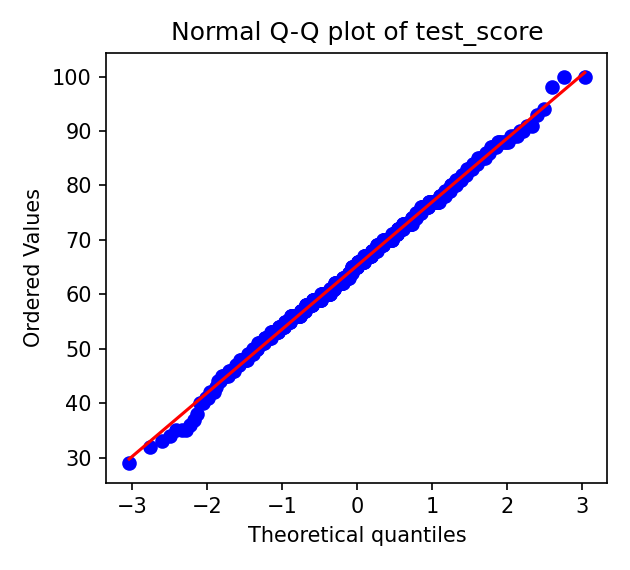
\includegraphics[width=\linewidth]{fig/qq.png}
\end{minipage}\hfill
\begin{minipage}{0.52\linewidth}
자료의 분위수를 정규분포 분위수에 대해 그립니다. \textbf{직선이면 정규근사가 적절}합니다. \nref{§5.5–5.6}
\begin{itemize}
\item 양 끝이 직선보다 바깥으로 휨: 꼬리가 두꺼움 (\term{heavy tails})
\item 안쪽으로 휨: 꼬리가 얇음
\item 한쪽만 휨: 비대칭 (\term{skew})
\end{itemize}
\aside{※ \code{test\_score}는 거의 직선이고, 끝의 계단 모양은 정수 점수 때문입니다.}
\end{minipage}

\begin{hypbox}
\begin{itemize}
\item \textbf{가설}: $H_0$: test\_score는 정규분포를 따른다.
\item \textbf{검증}: Q-Q plot (시각적) + Shapiro–Wilk (\code{scipy.stats.shapiro}) $p=0.47$ $\Rightarrow$ 기각하지 않음.
\item \textbf{의미}: 정규 가정을 쓰는 $t$-test 등을 써도 무리가 없습니다. 더 중요한 점: 표본이 크면 CLT 덕분에 \emph{평균}은 원자료가 정규가 아니어도 근사적으로 정규입니다 (4장).
\end{itemize}
\end{hypbox}

%=================================================
\section{groupby: 점추정과 신뢰구간}

\begin{codebox}
g = df.groupby("gender")["hired"].agg(["mean", "count"])
\end{codebox}
\begin{center}
\begin{tabular}{@{}l c c c c@{}}
\toprule
 & $n$ & 합격 & $\hat p$ & $\SE=\sqrt{\hat p(1-\hat p)/n}$ \\
\midrule
F & 313 & 68 & 0.217 & 0.023 \\
M & 287 & 125 & 0.436 & 0.029 \\
\bottomrule
\end{tabular}
\end{center}

\subsection{점추정}
각 지원자 $Y_i\sim\text{Bernoulli}(p)$. 추정량 $\hat p=\bar Y$ (표본비율).
\begin{itemize}
\item MoM: $\E[Y]=p$를 $\bar Y$로 바꿔 놓으면 $\hat p=\bar Y$. \nref{§4} \fwd{10장}
\item MLE도 같은 답. \nref{§6}
\item Unbiased: $\E[\hat p]=p$. $\Var(\hat p)=p(1-p)/n$.
\end{itemize}

\subsection{표본평균의 분포와 CLT}
같은 채용 과정에서 다른 313명의 여성이 지원했다면 $\hat p_F$는 조금 달랐을 것입니다. 이 ``표본마다 달라지는 분포''가 \term{sampling distribution}입니다. \nref{§7.1}
\[
\text{CLT:}\quad \bar X\ \approx\ N\!\left(\mu,\ \frac{\sigma^2}{n}\right)\qquad(n\text{이 크면, 원래 분포와 무관}).
\]
\aside{※ 정규자료면 정확히 $\bar X\sim N(\mu,\sigma^2/n)$. \nref{Cor 8.9} 아니면 CLT로 근사. \nref{§7.4}}\\
\aside{※ SD vs SE: SD는 \emph{개인}들이 얼마나 퍼져 있나 (0.41), SE는 \emph{추정값}이 표본마다 얼마나 흔들리나 (0.023). $\SE=\SD/\sqrt n$.}

\subsection{신뢰구간}
\[
\hat p\pm1.96\,\SE \qquad\Longrightarrow\qquad F:\ [0.172,\ 0.263],\quad M:\ [0.378,\ 0.493].
\]
두 그룹 차이: $\hat p_M-\hat p_F=0.218$, $\SE=\sqrt{0.023^2+0.029^2}=0.037$, 95\% CI $[0.145,\ 0.292]$.

\aside{※ 1.96은 $z_{0.025}$: 표준정규에서 가운데 95\% 면적의 경계 (3장). \nref{§9.4}}\\
\aside{※ 해석: ``이 방법으로 구간을 만들면 100번 중 약 95번은 진짜 $p$를 포함한다.'' 진짜 $p$가 이 구간에 있을 확률이 95\%라는 뜻은 아닙니다. \nref{§9.1}}\\
\aside{※ 평균일 때 $\sigma$를 모르고 $s$를 쓰면 1.96 대신 $t_{n-1,0.025}$를 씁니다. \nref{Thm 8.16, §9.3}}

\begin{hypbox}
\begin{itemize}
\item \textbf{추정}: $p_M-p_F$의 점추정 0.218, 95\% CI $[0.145, 0.292]$.
\item \textbf{CI로 하는 검증}: 구간에 0이 없으므로 $H_0: p_M=p_F$는 5\% 수준에서 기각됩니다. (CI와 양측검정은 같은 정보를 다른 형태로 보여 줍니다.)
\end{itemize}
\end{hypbox}

%=================================================
\section{가설검정}

\subsection{검정의 다섯 단계} \nref{§10.1} \fwd{11장}
\begin{enumerate}
\item 가설: $H_0$ (차이 없음) vs $H_1$ (차이 있음).
\item 유의수준 $\alpha$ (보통 0.05)를 미리 정함.
\item 검정통계량: $\dfrac{\text{추정값}-H_0\text{에서의 값}}{\SE}$. 거의 모든 검정이 이 모양입니다.
\item $H_0$에서의 분포 ($N(0,1)$, $t$, $\chi^2$)로 p-value 계산.
\item $p<\alpha$이면 $H_0$ 기각.
\end{enumerate}
\begin{center}
\begin{tabular}{@{}l c c@{}}
\toprule
 & $H_0$ 참 & $H_0$ 거짓 \\
\midrule
기각 & Type I error ($\alpha$) & 맞음 (power) \\
기각 안 함 & 맞음 & Type II error \\
\bottomrule
\end{tabular}
\end{center}
\aside{※ p-value $=P(\text{지금만큼 극단적인 결과}\mid H_0)$. ``$H_0$가 참일 확률''이 아닙니다. 또 $p>0.05$는 ``차이 없음''의 증명이 아니라 ``증거 부족''입니다.}

\subsection{예 1. 두 비율: $z$-test}
\textbf{가설} $H_0:p_M=p_F$, $H_1:p_M\ne p_F$.\\
\textbf{통계량} $H_0$에서는 두 확률이 같으므로 합친 비율 $\hat p=193/600=0.322$로 SE를 계산:
\[
z=\frac{0.436-0.217}{\sqrt{0.322\cdot0.678\,(1/287+1/313)}}=\frac{0.218}{0.0382}=5.72.
\]
\textbf{검증} $p=2\,P(Z>5.72)=1.1\times10^{-8}<0.05$ $\Rightarrow$ 기각.
\begin{codebox}
from statsmodels.stats.proportion import proportions\_ztest\\
proportions\_ztest([125, 68], [287, 313]) \hfill \# (5.72, 1.1e-08)
\end{codebox}

\subsection{예 2. 교차표: $\chi^2$ 독립성 검정}
\begin{codebox}
ct = pd.crosstab(df.gender, df.hired)\\
chi2, p, dof, expected = scipy.stats.chi2\_contingency(ct, correction=False)
\end{codebox}
\begin{center}
\begin{tabular}{@{}l c c c c@{}}
\toprule
 & 관측 0 & 관측 1 & 기대 0 & 기대 1 \\
\midrule
F & 245 & 68 & 212.3 & 100.7 \\
M & 162 & 125 & 194.7 & 92.3 \\
\bottomrule
\end{tabular}
\end{center}
기대빈도 = (행 합)(열 합)/$n$ = ``독립이라면 나왔을 숫자''. $\chi^2=\sum\frac{(O-E)^2}{E}=32.70$, 자유도 $(2-1)(2-1)=1$, $p=1.1\times10^{-8}$.\\
\aside{※ $\chi^2(r)$ = 표준정규 $r$개의 제곱합. \nref{Def 8.10} 그래서 $2\times2$ 표에서는 $\chi^2=z^2$ ($5.72^2=32.7$)입니다.}

\subsection{예 3. 두 평균: Welch $t$-test}
\textbf{질문}: 남성이 원래 점수가 높아서 많이 붙은 것일까?\\
\textbf{가설} $H_0:\mu_M=\mu_F$ (점수 평균이 같다).
\[
t=\frac{65.79-64.73}{\sqrt{11.39^2/279+11.89^2/303}}=\frac{1.06}{0.97}=1.10,\qquad p=0.27.
\]
\textbf{검증} 기각하지 않음. 점수 차이에 대한 증거가 없으므로 ``점수 때문''이라는 설명은 약합니다.
\begin{codebox}
scipy.stats.ttest\_ind(male\_scores, female\_scores, equal\_var=False)
\end{codebox}
\aside{※ 분산이 같다고 가정하면 pooled $t$, 아니면 Welch. 기본은 Welch가 안전합니다. \nref{§10.5.2–10.5.3}} \fwd{12장 검정 도구상자}

\begin{hypbox}
\begin{center}
\begin{tabular}{@{}l l l l@{}}
\toprule
질문 & $H_0$ & 통계량 & 결론 \\
\midrule
합격률이 성별로 다른가 & $p_M=p_F$ & $z=5.72$ & 기각 ($p\approx10^{-8}$) \\
성별과 합격이 독립인가 & 독립 & $\chi^2=32.7$ & 기각 \\
점수가 성별로 다른가 & $\mu_M=\mu_F$ & $t=1.10$ & 기각 못 함 ($p=0.27$) \\
\bottomrule
\end{tabular}
\end{center}
\end{hypbox}

%=================================================
\section{corr(): 산포도와 상관계수}

\begin{codebox}
df[["years\_experience","test\_score","hired"]].corr()
\end{codebox}
\begin{center}
\begin{tabular}{@{}l c c c@{}}
\toprule
 & experience & score & hired \\
\midrule
experience & 1 & 0.008 & 0.197 \\
score & 0.008 & 1 & 0.247 \\
hired & 0.197 & 0.247 & 1 \\
\bottomrule
\end{tabular}
\end{center}

\subsection{산포도}
두 수치 변수의 관계는 먼저 \term{scatter plot}으로 봅니다 (\code{df.plot.scatter("test\_score","hired")}). 볼 것: 방향(양/음), 형태(직선/곡선), 강도(점이 얼마나 모여 있나), 이탈값. 7장 그림 왼쪽이 \code{test\_score}–\code{hired}의 산포도입니다.

\subsection{상관계수 구하는 법}
\[
r=\text{평균}\big[(x\text{의 }z\text{-score})\times(y\text{의 }z\text{-score})\big]=\frac1n\sum_i\frac{x_i-\bar x}{\SD_x}\cdot\frac{y_i-\bar y}{\SD_y}.
\]
\begin{enumerate}
\item 두 변수를 각각 표준점수로 바꾼다 (SD는 $n$으로 나눈 것).
\item 짝끼리 곱한다. 둘 다 평균보다 크거나 둘 다 작으면 $+$, 엇갈리면 $-$.
\item 평균낸다.
\end{enumerate}
\begin{codebox}
zx = (x - x.mean())/x.std(ddof=0); zy = (y - y.mean())/y.std(ddof=0)\\
(zx * zy).mean() \hfill \# 0.2465 = df.corr()의 값
\end{codebox}
\aside{※ 노트에는 상관계수가 따로 정의되어 있지 않지만, 회귀 기울기 $\hat\beta=\frac{\text{cov}}{\text{var}}$에 같은 재료가 쓰입니다. $r=\frac{\text{cov}(x,y)}{\SD_x\SD_y}$. \nref{Remark 11.5}}

\subsection{성질}
\begin{itemize}
\item $-1\le r\le1$. $\pm1$이면 모든 점이 한 직선 위.
\item 단위와 무관: $x$를 $ax+b$ ($a>0$)로 바꿔도 $r$ 그대로 (점수를 10으로 나눠도 0.2465). $a<0$이면 부호만 바뀜.
\item 대칭: $r(x,y)=r(y,x)$.
\item 0/1 변수와의 상관도 같은 공식 (\term{point-biserial correlation}).
\end{itemize}

\subsection{유의사항}
\begin{itemize}
\item \textbf{직선 관계만 잰다.} $r\approx0$이어도 곡선 관계는 강할 수 있습니다 (Anscombe 2번 자료). \textbf{반드시 산포도를 먼저.} \nref{Ex 11.15}
\item \textbf{이탈값 한 점}이 $r$을 크게 바꿀 수 있습니다.
\item \textbf{상관은 인과가 아니다.} 제3의 변수(confounder)가 둘 다를 움직일 수 있습니다.
\item \textbf{평균끼리의 상관} (부서별 평균 등)은 개인 단위 상관보다 훨씬 강하게 나옵니다 (\term{ecological correlation}).
\item \textbf{범위 제한}: 점수 상위권만 뽑아서 보면 $r$이 작아집니다.
\item 측정오차는 $r$을 0 쪽으로 줄입니다 (1장).
\end{itemize}
\aside{※ experience–score $r=0.008$: 두 자격 변수는 사실상 무관합니다. 그래서 회귀에 같이 넣어도 서로 효과를 빼앗지 않습니다.}

\begin{hypbox}
\begin{itemize}
\item \textbf{추정}: 모집단 상관 $\rho$의 추정값 $r=0.247$ ($n=582$).
\item \textbf{가설}: $H_0:\rho=0$ (점수와 합격은 선형으로 무관).
\item \textbf{검증}: $t=\dfrac{r\sqrt{n-2}}{\sqrt{1-r^2}}=\dfrac{0.247\sqrt{580}}{\sqrt{1-0.061}}=6.13$, 자유도 $n-2$, $p=1.7\times10^{-9}$ $\Rightarrow$ 기각. (\code{scipy.stats.pearsonr})
\item experience–score: $r=0.008$, $p=0.85$ $\Rightarrow$ 기각 못 함.
\end{itemize}
\aside{※ 이 $t$는 8장의 기울기 $t$와 정확히 같은 값입니다. ``상관이 0''과 ``기울기가 0''은 같은 가설이기 때문입니다.}
\end{hypbox}

%=================================================
\section{회귀분석: 변수 간의 관계}

\subsection{평균의 그래프}
``점수가 $x$인 사람들의 평균 합격률''을 점수 구간별로 구해 이은 것이 \term{graph of averages}입니다.
\begin{codebox}
bins = pd.cut(d.test\_score, [0,40,50,55,60,65,70,75,80,90,101])\\
d.groupby(bins)["hired"].mean()
\end{codebox}
\begin{center}
\begin{tabular}{@{}l *{10}{c}@{}}
\toprule
점수 & $\le$40 & 40–50 & 50–55 & 55–60 & 60–65 & 65–70 & 70–75 & 75–80 & 80–90 & 90+ \\
$n$ & 12 & 42 & 55 & 101 & 83 & 103 & 72 & 60 & 47 & 7 \\
합격률 & .00 & .21 & .15 & .26 & .31 & .30 & .46 & .43 & .60 & .29 \\
\bottomrule
\end{tabular}
\end{center}
\textbf{회귀선 = 평균의 그래프를 직선으로 다듬은 것.} 평균의 그래프가 대략 직선이면 회귀선을 써도 됩니다.\\
\aside{※ 90점 이상의 .29는 7명뿐이라 매우 불안정합니다. 표본이 작은 구간은 믿지 마세요.}

\begin{center}
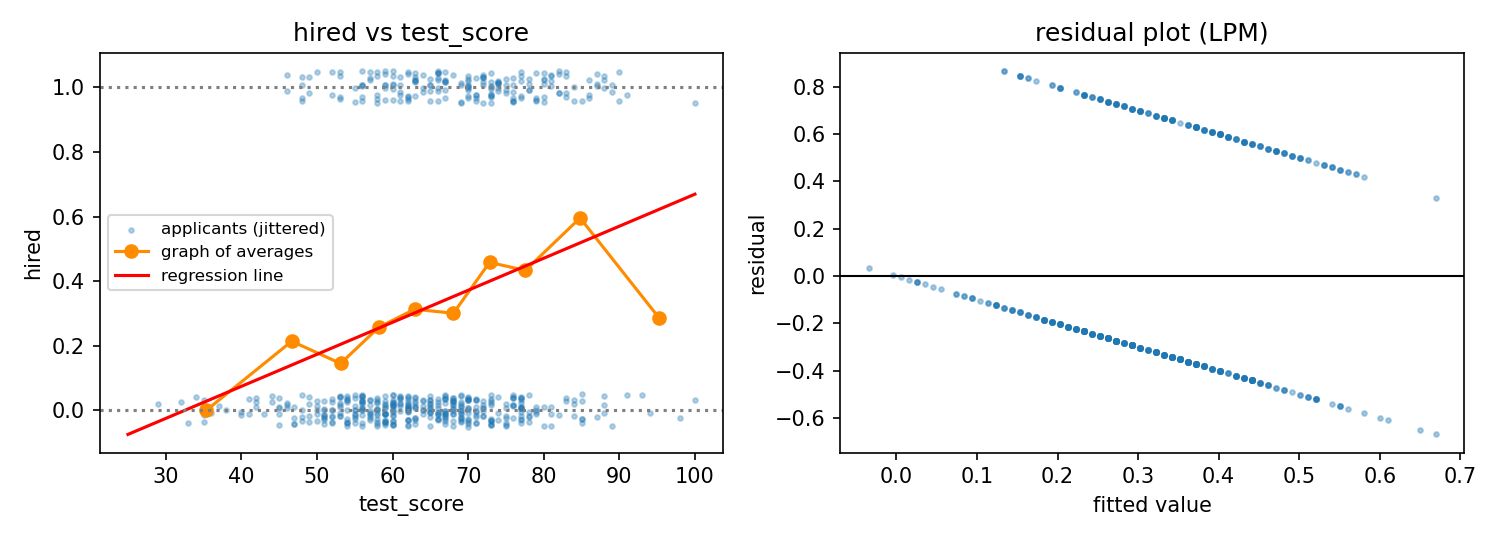
\includegraphics[width=\linewidth]{fig/reg.png}
\end{center}

\subsection{회귀선 구하는 법}
모형: $Y_i=\alpha+\beta x_i+\sigma Z_i$, $\E[Z_i]=0$, $\Var(Z_i)=1$. \nref{Def 11.1}\\
최소제곱 (잔차 제곱합 최소화)의 해 \nref{Thm 11.4}:
\[
\hat\beta=\frac{\sum(x_i-\bar x)(y_i-\bar y)}{\sum(x_i-\bar x)^2}=r\cdot\frac{\SD_y}{\SD_x},\qquad \hat\alpha=\bar y-\hat\beta\bar x.
\]
\textbf{기억하는 법}: $x$가 1 SD 늘면, $y$는 평균적으로 $r$ SD만큼 늘어난다. 회귀선은 점 $(\bar x,\bar y)$를 지납니다.

\begin{codebox}
smf.ols("hired \~{} test\_score", data=d).fit().params
\end{codebox}
손계산: $\bar x=65.24$, $\SD_x=11.65$, $\bar y=0.325$, $\SD_y=0.468$, $r=0.247$.
\[
\hat\beta=0.247\times\frac{0.468}{11.65}=0.0099,\qquad \hat\alpha=0.325-0.0099\times65.24=-0.322.
\]
해석: 점수 1점당 합격 확률 +1.0\%p, 10점당 +9.9\%p. 예측: 80점 $\to0.47$, 50점 $\to0.17$.\\
\aside{※ 30점 $\to-0.02$: 직선은 0 아래로 내려갑니다. 0/1 결과에 직선을 쓰는 LPM의 한계이고, 그래서 logistic regression을 보조로 씁니다 (이전 책 §7). 또한 자료 범위 밖으로 예측하는 \term{extrapolation}은 위험합니다.}

\subsection{회귀 효과 (regression effect)}
기울기를 SD 단위로 보면 $r$입니다. $|r|<1$이므로, \textbf{$x$에서 극단적인 사람의 $y$ 예측값은 덜 극단적}입니다. 이것이 \term{regression to the mean}입니다.

\textbf{$y$를 $x$로 예측 (hired $\sim$ score)}: 점수가 평균보다 2 SD 위 (88.5점)인 사람의 예측 합격률은 $y$ 평균보다 $r\times2=0.49$ SD 위, 즉 $0.325+0.49\times0.468=0.56$. 2 SD가 아니라 0.49 SD.

\textbf{$x$를 $y$로 예측 (score $\sim$ hired)}: 합격자 ($y=1$, $z_y=1.44$)의 예측 점수는 평균보다 $r\times1.44=0.36$ SD 위, 즉 $65.24+0.36\times11.65=69.4$점. 실제 합격자 평균도 69.4점입니다.\\
\aside{※ 정확히 일치하는 이유: 설명변수가 0/1이면 회귀 예측값은 그 그룹의 평균입니다 (이전 책 연습문제 6).}

\begin{minipage}{0.46\linewidth}
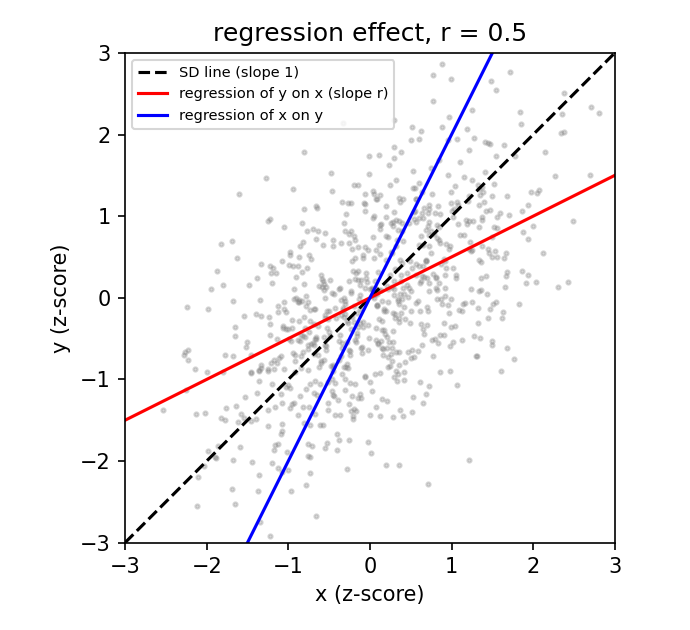
\includegraphics[width=\linewidth]{fig/regeffect.png}
\end{minipage}\hfill
\begin{minipage}{0.5\linewidth}
\textbf{두 개의 회귀선} (표준화한 자료, $r=0.5$ 예시):
\begin{itemize}
\item \textbf{SD line} (점선, 기울기 1): 구름의 장축. 눈으로 보면 이 선이 ``맞는 선'' 같지만 예측선이 아닙니다.
\item \textbf{$y$ on $x$} (빨강): 기울기 $r$. SD line보다 \emph{눕습니다}.
\item \textbf{$x$ on $y$} (파랑): $x=r\,y$. SD line보다 \emph{섭니다}.
\end{itemize}
원래 단위에서 기울기 곱: $\hat\beta_{y|x}\cdot\hat\beta_{x|y}=r\frac{\SD_y}{\SD_x}\cdot r\frac{\SD_x}{\SD_y}=r^2$. 여기서는 $0.0099\times6.13=0.061=0.247^2$.\\
\aside{※ 그래서 $y$를 $x$로 예측한 식을 거꾸로 풀어 $x$를 예측하면 \emph{틀립니다}. 방향마다 회귀를 따로 해야 합니다.}
\end{minipage}

\begin{keybox}{회귀의 오류 (regression fallacy)}
시험 1등이 다음 시험에서 성적이 떨어지는 것은 대개 ``자만해서''가 아니라 회귀 효과입니다. 1등에는 실력 + 행운(측정오차)이 섞여 있고, 다음 시험에서는 행운이 반복되지 않습니다. 회귀 효과에 인과적 설명을 붙이는 것이 \term{regression fallacy}입니다.
\end{keybox}

\begin{hypbox}
\begin{itemize}
\item \textbf{추정}: $\hat\beta=0.0099$ (점수 1점당 합격 확률 +1\%p).
\item 추정량의 성질: $\hat\alpha,\hat\beta$는 unbiased이고 $\Var(\hat\beta)=\dfrac{\sigma^2}{\sum(x_i-\bar x)^2}$. \nref{Thm 11.6}\\
\aside{※ $x$가 넓게 퍼져 있을수록 기울기를 정확하게 추정합니다.}
\item 검정은 오차 $\sigma$를 추정한 뒤에 할 수 있습니다 $\to$ 8장.
\end{itemize}
\end{hypbox}

%=================================================
\section{회귀분석의 오차}

\subsection{실제값과 추정치의 차이: 잔차}
\begin{codebox}
fit = smf.ols("hired \~{} test\_score", data=d).fit()\\
fit.fittedvalues \hfill \# 추정치 $\hat y_i$\\
fit.resid \hfill \# 잔차 $e_i=y_i-\hat y_i$
\end{codebox}
\begin{itemize}
\item \term{Fitted value} $\hat y_i=\hat\alpha+\hat\beta x_i$. \nref{Def 11.10}
\item \term{Error} $Y_i-\alpha-\beta x_i$: 진짜 직선에서의 차이. 관측 불가.\\
\term{Residual} $e_i=y_i-\hat y_i$: 추정한 직선에서의 차이. 관측 가능, error의 추정치. \nref{Def 11.11}
\item 잔차는 항상 $\sum e_i=0$이고 $x$와 상관이 0입니다 (최소제곱의 normal equation).
\end{itemize}

\subsection{RMSE: 상관계수로 계산하기}
회귀선의 전형적인 오차 크기 = 잔차의 RMS:
\[
\text{RMSE}=\text{RMS}(e_1,\dots,e_n)=\sqrt{1-r^2}\cdot\SD_y.
\]
\begin{center}
\begin{tabular}{@{}l c@{}}
\toprule
직접 계산 \code{np.sqrt((fit.resid**2).mean())} & 0.4538 \\
공식 $\sqrt{1-0.247^2}\times0.468$ & 0.4538 \\
\bottomrule
\end{tabular}
\end{center}
\textbf{해석}:
\begin{itemize}
\item $r=0$: RMSE $=\SD_y$. $x$가 아무 도움이 안 되므로 그냥 평균으로 예측하는 것과 같음.
\item $r=\pm1$: RMSE $=0$. 완벽한 예측.
\item 여기서는 $\sqrt{1-0.061}=0.97$: 점수를 알아도 예측 오차가 3\%만 줄어듭니다. 점수는 \emph{유의한} 변수지만 혼자서는 합격을 잘 \emph{예측}하지 못합니다.
\end{itemize}
\aside{※ $r^2=0.061$은 \term{$R^2$} (설명된 분산 비율)와 같습니다. 유의성($p$)과 예측력($R^2$)은 다른 질문입니다.}\\
\aside{※ 증명 스케치: $\sum e_i^2=\sum(y_i-\bar y)^2-\hat\beta^2\sum(x_i-\bar x)^2$ \nref{Prop 11.13 증명}에 $\hat\beta=r\SD_y/\SD_x$를 넣으면 $n\SD_y^2(1-r^2)$.}\\
\aside{※ 사용법: 정규 모양이면 회귀선 $\pm1$ RMSE 안에 약 68\%, $\pm2$ RMSE 안에 약 95\%의 점이 들어갑니다 (3장의 정규근사를 잔차에 적용).}

\subsection{$\sigma$의 추정과 자유도 $n-2$}
\[
\hat\sigma^2=\frac{\text{RSS}}{n-2}=\frac1{n-2}\sum e_i^2\qquad(\text{unbiased}).\quad \nref{Prop 11.13}
\]
$\alpha,\beta$ 두 개를 데이터로 추정했기 때문에 자유도가 2 줄어듭니다 (2장의 $n-1$과 같은 원리). 여기서 $\hat\sigma=0.4546$ vs RMSE 0.4538.

\subsection{잔차도 (residual plot)}
$x$축에 $\hat y$ (또는 $x$), $y$축에 잔차를 그립니다 (7장 그림 오른쪽). \textbf{좋은 잔차도 = 0 주위에 아무 패턴 없이 고르게 흩어진 띠.} \nref{Ex 11.14}
\begin{center}
\begin{tabular}{@{}p{5cm} p{9cm}@{}}
\toprule
보이는 모양 & 의미 \\
\midrule
패턴 없는 수평 띠 & 직선 모형 적절 \\
곡선 (U자 등) & 관계가 비선형 $\to$ 변수 변환, 다항식 \\
부채꼴 (점점 넓어짐) & 분산이 $x$에 따라 다름 (\term{heteroskedasticity}) $\to$ robust SE \\
멀리 떨어진 점 & 이탈값, 영향점 $\to$ 빼고 다시 확인 \\
\bottomrule
\end{tabular}
\end{center}
\aside{※ 우리 그림의 두 줄 띠는 $y$가 0/1이라 생기는 모양 ($y=1$이면 $1-\hat y$, $y=0$이면 $-\hat y$)이고, LPM에서는 정상입니다. 대신 분산이 $\hat y(1-\hat y)$로 변하므로 robust SE를 씁니다.}\\
\aside{※ 요약통계(평균, SD, $r$)가 같아도 그림은 전혀 다를 수 있습니다 (Anscombe). 숫자만 보지 말고 항상 산포도와 잔차도를 그립니다. \nref{Ex 11.15}}

\begin{hypbox}
\begin{itemize}
\item \textbf{가설}: $H_0:\beta=0$ (점수는 합격 확률과 선형 관계가 없다).
\item \textbf{통계량}: $\SE(\hat\beta)=\hat\sigma/\sqrt{\sum(x_i-\bar x)^2}=0.00162$, \quad $t=\hat\beta/\SE=0.00991/0.00162=6.13$.\\
정규 오차 가정에서 $t\sim t(n-2)$. \nref{Thm 11.18}
\item \textbf{검증}: $p=1.7\times10^{-9}$ $\Rightarrow$ 기각. 95\% CI $[0.0067,\ 0.0131]$ (0 미포함).
\item 6장의 $r$ 검정과 같은 $t=6.13$입니다.
\end{itemize}
\aside{※ \fwd{13장} 이 틀이 그대로 다중회귀로 확장됩니다: \code{hired \~{} C(gender) + test\_score + ...}에서 성별 계수의 $t$-test가 ``점수 등을 통제해도 성별 차이가 있는가''의 검증입니다 (이전 책 §6).}
\end{hypbox}

%=================================================
\section{추정량 깊이 보기}
\linkup{2장 SE, 4장 점추정}

\subsection{추정량(estimator)과 추정값(estimate)}
\begin{itemize}
\item \term{Estimator} $\hat\theta=T(X_1,\dots,X_n)$: 데이터를 넣으면 숫자를 내는 \emph{규칙(함수)}. 확률변수입니다.
\item \term{Estimate} $T(x_1,\dots,x_n)$: 실제 데이터를 넣어 나온 \emph{숫자}. \nref{Def 3.6}
\end{itemize}
\aside{※ pandas로 비유하면: 추정량 = \code{lambda d: d.groupby("gender").hired.mean()}, 추정값 = 그 함수를 \code{df}에 적용한 결과 0.217.}\\
\aside{※ 모르는 값의 \emph{함수} $g(\theta)$도 $g(\hat\theta)$로 추정합니다. \nref{Ex 3.7} 예: 여성의 합격 odds $p/(1-p)$의 추정값 $=0.217/0.783=0.278$. MLE는 이렇게 변환해도 여전히 MLE입니다 (\term{invariance}). \nref{§6.3}}

\subsection{표본분포를 눈으로 보기: bootstrap}
추정량이 확률변수라는 것을 pandas로 직접 확인할 수 있습니다. 데이터에서 \emph{복원추출}로 같은 크기의 표본을 계속 다시 뽑아, 그때마다 추정값을 계산합니다.
\begin{codebox}
diffs = []\\
for b in range(2000):\\
\ \ \ \ bs = df.sample(frac=1, replace=True)\\
\ \ \ \ m = bs.groupby("gender").hired.mean()\\
\ \ \ \ diffs.append(m["M"] - m["F"])\\
np.std(diffs) \hfill \# 0.0385\\
np.percentile(diffs, [2.5, 97.5]) \hfill \# [0.144, 0.293]
\end{codebox}
\begin{center}
\begin{tabular}{@{}l c c@{}}
\toprule
$\hat p_M-\hat p_F$ & SE & 95\% 구간 \\
\midrule
공식 (4장) & 0.0374 & $[0.145,\ 0.292]$ \\
Bootstrap (2000회) & 0.0385 & $[0.144,\ 0.293]$ \\
\bottomrule
\end{tabular}
\end{center}
\aside{※ 공식과 거의 같습니다. 공식이 없는 추정량(중앙값, disparate impact ratio 등)의 SE도 같은 코드로 구할 수 있다는 것이 bootstrap의 힘입니다. 노트의 ``시뮬레이션으로 표본분포 근사''와 같은 생각입니다. \nref{§7.3}}

\subsection{좋은 추정량의 기준}
\begin{center}
\begin{tabular}{@{}p{2.8cm} p{5.2cm} p{6.2cm}@{}}
\toprule
기준 & 정의 & 뜻 \\
\midrule
\term{Bias} & $\E[\hat\theta]-\theta$ \nref{Def 7.2} & 평균적으로 과녁 중심을 맞히는가 \\
\term{Variance} & $\Var(\hat\theta)$ & 얼마나 흩어지는가 \\
\term{Standard error} & $\sqrt{\Var(\hat\theta)}$의 추정값 & 보고용 흔들림 크기 \\
\term{MSE} & $\E[(\hat\theta-\theta)^2]$ \nref{Def 7.3} & 전체 오차 = $\Var+\text{bias}^2$ \nref{Prop 7.4} \\
\term{Consistency} & $n\to\infty$이면 $\hat\theta\to\theta$ & 데이터가 많으면 결국 맞힌다 \\
\bottomrule
\end{tabular}
\end{center}
\aside{※ 과녁 비유: bias = 화살 무리의 중심이 과녁 중심에서 벗어난 정도, variance = 화살 무리의 퍼짐. MSE는 둘 다 합친 것이라, 약간의 bias를 감수하고 분산을 크게 줄이면 MSE가 더 작아질 수도 있습니다 (Ridge 회귀의 원리).}

\textbf{예: 분산 추정량의 bias를 시뮬레이션으로 확인} \linkup{2장 자유도}\\
$N(65,\,11.66^2)$에서 $n=5$짜리 표본을 10만 번 뽑아 두 분산 추정량의 평균을 냈습니다.
\begin{center}
\begin{tabular}{@{}l c c@{}}
\toprule
추정량 & 10만 번 평균 & 진짜 $\sigma^2=135.96$ 대비 \\
\midrule
$\frac1n\sum(x_i-\bar x)^2$ (\code{ddof=0}) & 108.4 & 약 $\frac45$ (bias $\approx-27$) \\
$\frac1{n-1}\sum(x_i-\bar x)^2$ (\code{ddof=1}) & 135.5 & 거의 같음 (unbiased) \\
\bottomrule
\end{tabular}
\end{center}
\aside{※ 이론값 $\frac{n-1}n\sigma^2=\frac45\times135.96=108.8$과 일치합니다. $n=582$에서는 $\frac{581}{582}$라 무시할 만합니다.}

\textbf{예: $\bar X$의 MSE} \nref{Ex 7.5}\\
$\E[\bar X]=\mu$ (unbiased), $\Var(\bar X)=\sigma^2/n$ $\Rightarrow$ MSE $=\sigma^2/n\to0$ (consistent). 표본을 4배로 늘리면 SE가 절반이 됩니다 ($\sqrt n$ 법칙).

\begin{hypbox}
\textbf{추정의 보고 형식}: ``점추정값 (SE)'' 또는 ``점추정값, 95\% CI''. 숫자 하나만 보고하면 그것이 얼마나 믿을 만한지 알 수 없습니다.\\
예: ``남성의 합격률이 21.8\%p 높다 (SE 3.7\%p, 95\% CI 14.5–29.2\%p).''
\end{hypbox}

%=================================================
\section{추정량 만들기: 적률법(MoM)과 최우추정(MLE)}
\linkup{4장 점추정}
\aside{※ ``momentum''이 아니라 \term{moment}(적률)입니다. 물리학의 moment(모멘트)와 같은 단어로, 분포의 ``무게중심''(1차), ``관성''(2차)이라는 비유에서 왔습니다.}

\subsection{적률 (moment)}
\begin{itemize}
\item $k$차 \term{moment}: $\E[X^k]$. 1차 moment는 평균. \nref{Def 4.1}
\item $k$차 \term{empirical moment}: $M_k=\frac1n\sum X_i^k$. pandas로는 \code{(df.col**k).mean()}. \nref{Def 4.2}
\item 분산은 1, 2차 moment로 표현됩니다: $\Var(X)=\E[X^2]-(\E[X])^2$.
\end{itemize}

\subsection{MoM 절차} \nref{Def 4.3}
\begin{enumerate}
\item 모형을 정한다: $X_i\sim f(x;\theta)$, parameter가 $k$개.
\item 이론 moment $\E[X],\E[X^2],\dots,\E[X^k]$을 $\theta$의 식으로 쓴다.
\item 이론 moment $=$ 표본 moment로 놓는다 ($k$개의 방정식).
\item $\theta$에 대해 푼다.
\end{enumerate}

\textbf{예 1. Bernoulli (합격 여부)}: $\E[Y]=p$ $\Rightarrow$ $\hat p=M_1=\bar Y$. 4장의 \code{groupby().mean()}.

\textbf{예 2. Normal (\code{test\_score})} \nref{Ex 4.6}: parameter 2개 $\Rightarrow$ 방정식 2개.
\[
\hat\mu=M_1=65.24,\qquad \hat\mu^2+\hat\sigma^2=M_2\ \Rightarrow\ \hat\sigma^2=M_2-M_1^2=\tfrac1n\textstyle\sum(x_i-\bar x)^2=135.66.
\]
\aside{※ MoM 분산은 $n$으로 나눈 것 (2장 \code{ddof=0})이라 약간의 bias가 있습니다.}

\textbf{예 3. Exponential (대기 시간 등)} \nref{Ex 4.5}: $\E[X]=1/\theta$ $\Rightarrow$ $\hat\theta=1/\bar X$.

\textbf{예 4. Poisson (\code{years\_experience}를 셈 자료로 보면)}: $\E[X]=\lambda$, $\Var(X)=\lambda$.
\begin{codebox}
e = df.years\_experience\\
e.mean(), e.var() \hfill \# 4.455, 3.851
\end{codebox}
1차 moment로 풀면 $\hat\lambda=4.455$, 2차 moment(분산)로 풀면 $\hat\lambda=3.851$. \textbf{같은 MoM인데 답이 다릅니다.}\\
\aside{※ 어떤 moment를 쓰느냐에 따라 MoM 답이 달라질 수 있다는 것이 MoM의 약점입니다 (보통 낮은 차수부터 씀). \nref{Remark 4.4}}\\
\aside{※ 동시에 \emph{모형 점검} 도구이기도 합니다: Poisson이면 평균 $=$ 분산이어야 하는데 분산이 더 작으므로 (\term{underdispersion}) Poisson 모형이 딱 맞지는 않는다는 신호입니다.}

\subsection{MLE 절차} \nref{§6.2}
\begin{enumerate}
\item Likelihood $L(\theta)=\prod_i f(x_i;\theta)$: ``$\theta$일 때 지금 데이터가 나올 확률''.
\item 로그: $\ell(\theta)=\sum_i\log f(x_i;\theta)$ (곱 $\to$ 합).
\item $\ell'(\theta)=0$을 푼다.
\item $\ell''(\theta)<0$으로 최댓값 확인. (경계에서 최대일 수도 있음: Uniform$(0,\theta)$ \nref{§6.5})
\end{enumerate}

\textbf{예. Poisson}: $\ell(\lambda)=-n\lambda+(\sum x_i)\log\lambda+C$, $\ell'=-n+\sum x_i/\lambda=0$ $\Rightarrow$ $\hat\lambda=\bar x=4.455$. 1차 MoM과 같습니다.\\
\textbf{예. Bernoulli}: $\hat p=k/n$ (이전 책 §4). \textbf{예. Normal}: $\hat\mu=\bar x$, $\hat\sigma^2=\frac1n\sum(x_i-\bar x)^2$ (MoM과 같음).

\subsection{MoM vs MLE: 언제 무엇을}
\begin{center}
\begin{tabular}{@{}p{3cm} p{5.5cm} p{5.5cm}@{}}
\toprule
 & MoM & MLE \\
\midrule
필요한 것 & moment 식만 & 분포 전체 \\
계산 & 방정식 풀기 (보통 쉬움) & 미분 또는 수치 최적화 \\
답의 유일성 & moment 선택에 따라 다를 수 있음 & 하나 (보통) \\
정확도 & 괜찮음 & 큰 표본에서 분산이 가장 작음 \\
변환 & -- & $g(\hat\theta)$도 MLE (invariance) \\
쓰이는 곳 & OLS, 초기값, 빠른 계산 & logistic 회귀, 대부분의 모형 \\
\bottomrule
\end{tabular}
\end{center}
\aside{※ 여러 단순한 모형(Bernoulli, Poisson, Normal 평균)에서는 두 방법이 같은 답을 줍니다. 다른 경우에는 보통 MLE를 씁니다.}\\
\aside{※ 회귀와의 연결 \fwd{13장}: OLS의 normal equation $\frac1n\sum x_i(y_i-\hat y_i)=0$은 moment 조건 $\E[X\varepsilon]=0$의 표본 버전입니다 (MoM). 오차가 정규분포면 OLS는 MLE이기도 합니다. \nref{Prop 11.17}}

\begin{hypbox}
\textbf{추정 $\to$ 검정의 연결}: MLE는 큰 표본에서 근사적으로 정규분포 $\hat\theta\approx N(\theta,\SE^2)$를 따릅니다. 그래서 거의 모든 검정통계량이 $\dfrac{\hat\theta-\theta_0}{\SE}\approx N(0,1)$ 꼴이 되고, 이것이 다음 두 장의 출발점입니다.
\end{hypbox}

%=================================================
\section{가설 세우기와 검증 설계}
\linkup{5장 검정의 다섯 단계}

\subsection{가설 세우는 법}
\begin{enumerate}
\item \textbf{질문을 parameter로 바꾼다}: ``여성이 불리한가?'' $\to$ $p_F$와 $p_M$의 비교.
\item \textbf{$H_0$는 ``효과 없음'' (등호)}: $H_0: p_M-p_F=0$. 귀류법의 ``가정''에 해당합니다.
\item \textbf{$H_1$의 방향을 데이터 보기 전에 정한다}:
\begin{itemize}
\item 양측 $H_1:p_M\ne p_F$: 어느 쪽이든 차이를 찾을 때 (기본값).
\item 단측 $H_1:p_M>p_F$: 한쪽 방향만 의미 있을 때. 노트 Ex 10.4–10.5 (신약이 \emph{늘렸는가}). \nref{Ex 10.4}
\end{itemize}
\aside{※ 단측 p-value는 양측의 절반이라 기각하기 쉽습니다. 그래서 데이터를 본 뒤 단측으로 바꾸는 것은 반칙입니다. 노트도 이 점을 경고합니다. \nref{§10.2}}
\item \textbf{$\alpha$를 미리 정한다} (보통 0.05).
\end{enumerate}

\subsection{기각 판단의 두 방법}
\begin{center}
\begin{tabular}{@{}p{3.4cm} p{5.2cm} p{5.6cm}@{}}
\toprule
 & 기각역 (critical region) \nref{Def 10.2} & p-value \nref{Def 10.3} \\
\midrule
방법 & $|z|\ge1.96$이면 기각 & $p=P(|Z|\ge|z_{\text{obs}}|)\le\alpha$이면 기각 \\
장점 & 데이터를 보기 전에 기준이 정해짐 & 어떤 $\alpha$에서 기각되는지 다 알려줌 \\
예 ($z=5.72$) & $5.72>1.96$ $\Rightarrow$ 기각 & $p=1.1\times10^{-8}$ \\
\bottomrule
\end{tabular}
\end{center}
\aside{※ 두 방법은 항상 같은 결론을 줍니다. 보고할 때는 p-value와 효과 크기를 함께 씁니다.}

\subsection{신뢰구간과 검정은 같은 동전의 양면} \nref{§9.3}
노트의 \term{pivot}: 분포가 $\theta$와 무관하게 완전히 알려진 양. 예: $\frac{\bar X-\mu}{S/\sqrt n}\sim t(n-1)$.
\begin{itemize}
\item pivot을 $\theta$에 대해 풀면 $\to$ \textbf{신뢰구간}.
\item pivot에 $\theta=\theta_0$를 넣으면 $\to$ \textbf{검정통계량}.
\end{itemize}
그래서 ``95\% CI에 $\theta_0$가 없다'' $\iff$ ``$\alpha=0.05$ 양측검정에서 $H_0:\theta=\theta_0$ 기각''.

\subsection{두 종류의 오류와 검정력}
\begin{itemize}
\item \term{Type I error}: 참인 $H_0$를 기각 (거짓 경보). 확률 $\le\alpha$로 \emph{우리가 통제}합니다. \nref{Def 10.1}
\item \term{Type II error}: 거짓인 $H_0$를 기각 못 함 (놓침). \nref{Def 10.9}
\item \term{Power} $=1-P(\text{Type II})$: 진짜 효과가 있을 때 찾아낼 확률. \nref{Def 10.10}
\end{itemize}
검정력을 키우는 것: 큰 표본 $n$, 큰 효과, 작은 잡음 $\sigma$, 큰 $\alpha$, (정당한 경우) 단측검정.

\begin{codebox}
from statsmodels.stats.power import NormalIndPower\\
from statsmodels.stats.proportion import proportion\_effectsize\\
es = proportion\_effectsize(0.27, 0.22) \hfill \# 5\%p 차이\\
NormalIndPower().power(es, nobs1=300, alpha=0.05) \hfill \# 0.30\\
NormalIndPower().solve\_power(es, power=0.8, alpha=0.05) \hfill \# 그룹당 1159명
\end{codebox}
\textbf{해석}: 그룹당 300명이면 22\% vs 27\% (5\%p) 차이는 \textbf{70\% 확률로 놓칩니다}. 실제 격차 21.8\%p는 검정력이 거의 1이라 확실히 잡힙니다.\\
\aside{※ 그래서 Marketing 남성 61명처럼 작은 그룹에서 ``유의하지 않음''이 나오면 ``차이 없음''이 아니라 ``검정력이 부족함''일 가능성이 큽니다 (5장 주의, 이전 책 Bayesian 장).}

\subsection{검증에서 흔한 실수}
\begin{itemize}
\item \textbf{p-value 오해}: $P(\text{data}\mid H_0)\ne P(H_0\mid\text{data})$. 노트도 Bayes 정리로 이 점을 보여 줍니다. \nref{§10.3}
\item \textbf{통계적 유의성 $\ne$ 실질적 중요성}: $n$이 아주 크면 0.1\%p 차이도 유의합니다. 효과 크기를 함께 보고합니다.
\item \textbf{다중검정}: 부서 $\times$ 학위 $\times$ 경력으로 20개 그룹을 검정하면 우연히 하나쯤 $p<0.05$가 나옵니다. Bonferroni: 각 검정을 $\alpha/m$ 기준으로.
\item \textbf{p-hacking}: 원하는 결과가 나올 때까지 변수, 그룹, 검정을 바꾸는 것. 분석 계획을 먼저 정하고, 바꿨다면 모두 보고합니다.
\item \textbf{가정 무시}: 각 검정은 독립성, 표본 크기 등의 가정이 있습니다 (다음 장).
\end{itemize}

%=================================================
\section{검정 도구상자: 어떤 검정을 언제 쓰나}
\linkup{5장의 $z$-test, $\chi^2$, $t$-test}

\subsection{고르는 법: 세 가지 질문}
\begin{enumerate}
\item \textbf{결과 변수의 종류는?} 수치 (평균 비교) / 범주 (비율·빈도 비교)
\item \textbf{그룹이 몇 개?} 하나 (기준값과 비교) / 둘 / 셋 이상
\item \textbf{표본이 독립인가, 짝지어져 있는가?} (같은 사람을 두 번 쟀는가)
\end{enumerate}

\begin{center}\small
\begin{tabular}{@{}p{2.4cm} p{2.6cm} p{4.4cm} p{4.6cm}@{}}
\toprule
결과 & 비교 & 검정 & \code{scipy.stats} / statsmodels \\
\midrule
수치 & 1그룹 vs 기준값 & ① one-sample $z$ ($\sigma$ 앎) / ② $t$ & \code{ttest\_1samp} \\
수치 & 2그룹, 독립 & ⑤ two-sample $z$, pooled $t$, Welch $t$ & \code{ttest\_ind(equal\_var=...)} \\
수치 & 2번 측정, 짝 & ⑥ paired $t$ & \code{ttest\_rel} \\
수치 & 3그룹 이상 & ⑪ ANOVA $F$ & \code{f\_oneway} \\
수치 & 분산 & ⑩ $\chi^2$ 분산 검정/구간 & \code{chi2.ppf} \\
0/1 & 1그룹 vs 기준값 & ③ one-sample 비율 $z$ & \code{proportions\_ztest} \\
0/1 & 2그룹 & ④ two-sample 비율 $z$ & \code{proportions\_ztest} \\
범주 & 1변수 vs 기대분포 & ⑦ $\chi^2$ 적합도 & \code{chisquare} \\
범주$\times$범주 & 교차표 & ⑧ $\chi^2$ 독립성 & \code{chi2\_contingency} \\
범주$\times$범주 & 칸이 작음 & ⑨ Fisher exact & \code{fisher\_exact} \\
아무거나 & 여러 변수 통제 & ⑫ 회귀 계수 $t$ / $F$ & \code{smf.ols(...).summary()} \\
아무거나 & 분포 가정 없이 & ⑬ permutation, bootstrap & 직접 구현 \\
\bottomrule
\end{tabular}
\end{center}
\aside{※ 모든 검정이 같은 뼈대: (추정값 $-$ $H_0$ 값)/SE, 또는 (관측 $-$ 기대)$^2$/기대. 다른 것은 \emph{추정 대상}과 \emph{$H_0$에서의 분포} ($N(0,1)$, $t$, $\chi^2$, $F$)뿐입니다.}

\subsection*{① One-sample $z$-test: $\sigma$를 알 때 평균} \nref{Ex 10.4–10.5}
\addcontentsline{toc}{subsection}{① One-sample $z$-test: $\sigma$를 알 때 평균}
\begin{itemize}
\item \textbf{언제}: 모집단 SD $\sigma$가 알려져 있을 때 (드묾. 예: 시험 출제기관이 SD를 공표).
\item \textbf{가설}: $H_0:\mu=\mu_0$. \quad \textbf{통계량}: $z=\dfrac{\bar x-\mu_0}{\sigma/\sqrt n}\overset{H_0}\sim N(0,1)$.
\item \textbf{예}: ``이 시험의 평균은 64점, SD 12점''이라고 공표되었다면, 우리 지원자는 평균과 다른가? $z=\frac{65.24-64}{12/\sqrt{582}}=2.48$, $p=0.013$ $\Rightarrow$ 기각. 우리 지원자 풀은 평균보다 약간 높습니다.
\end{itemize}

\subsection*{② One-sample $t$-test: $\sigma$를 모를 때 평균} \nref{Ex 10.6, Thm 8.16}
\addcontentsline{toc}{subsection}{② One-sample $t$-test: $\sigma$를 모를 때 평균}
\begin{itemize}
\item \textbf{언제}: 대부분의 실제 상황 ($\sigma$를 $s$로 추정).
\item \textbf{통계량}: $t=\dfrac{\bar x-\mu_0}{s/\sqrt n}\overset{H_0}\sim t(n-1)$. \aside{$\sigma$를 추정한 대가로 꼬리가 두꺼운 $t$분포를 씁니다.}
\item \textbf{코드}: \code{st.ttest\_1samp(d.test\_score, 64)} $\to$ $t=2.56$, $p=0.011$.
\item \textbf{가정}: 독립, 정규 (또는 $n$이 커서 CLT).
\end{itemize}
\aside{※ \linkup{3장} $n$이 크면 $t(n-1)\approx N(0,1)$: $t_{581,0.025}=1.964$ vs $z_{0.025}=1.960$. $n$이 작을 때만 차이가 중요합니다 (예: $t_{9,0.025}=2.262$).}

\subsection*{③ One-sample 비율 $z$-test}
\addcontentsline{toc}{subsection}{③ One-sample 비율 $z$-test}
\begin{itemize}
\item \textbf{언제}: 0/1 결과의 비율이 기준값과 다른가.
\item \textbf{통계량}: $z=\dfrac{\hat p-p_0}{\sqrt{p_0(1-p_0)/n}}$. \aside{SE에 $H_0$의 $p_0$를 씁니다.}
\item \textbf{예}: ``업계 평균 합격률 30\%''와 다른가? $\hat p=0.322$, $z=\frac{0.0217}{\sqrt{0.3\cdot0.7/600}}=1.16$, $p=0.25$ $\Rightarrow$ 기각 못 함.
\item \textbf{가정}: $np_0\ge10$, $n(1-p_0)\ge10$ 정도 (정규근사가 맞으려면).
\end{itemize}

\subsection*{④ Two-sample 비율 $z$-test} \linkup{5장 예 1}
\addcontentsline{toc}{subsection}{④ Two-sample 비율 $z$-test}
5장에서 한 성별 합격률 비교 ($z=5.72$). SE에 합친 비율 $\hat p$를 쓰는 이유: $H_0$에서는 두 그룹의 $p$가 같다고 가정하기 때문.\\
\aside{※ 신뢰구간을 만들 때는 $H_0$를 가정하지 않으므로 그룹별 $\hat p$로 SE를 계산합니다 (4장의 0.0374 vs 검정의 0.0382).}

\subsection*{⑤ Two-sample 평균: $z$ / pooled $t$ / Welch $t$} \nref{§10.5}
\addcontentsline{toc}{subsection}{⑤ Two-sample 평균: $z$ / pooled $t$ / Welch $t$}
\begin{center}
\begin{tabular}{@{}l l l@{}}
\toprule
검정 & 가정 & SE \\
\midrule
two-sample $z$ & $\sigma_1,\sigma_2$를 앎 & $\sqrt{\sigma_1^2/n_1+\sigma_2^2/n_2}$ \\
pooled $t$ & $\sigma_1=\sigma_2$ (모름) & $s_p\sqrt{1/n_1+1/n_2}$, df $n_1+n_2-2$ \\
Welch $t$ & 분산이 달라도 됨 & $\sqrt{s_1^2/n_1+s_2^2/n_2}$, df 근사 \\
\bottomrule
\end{tabular}
\end{center}
\textbf{예} (점수, 남 vs 여): pooled $t=1.099$ ($p=0.272$, $s_p=11.66$), Welch $t=1.101$ ($p=0.272$). 분산비 $0.92$로 비슷해서 거의 같습니다.\\
\aside{※ 분산이 크게 다르고 표본 크기도 다르면 pooled $t$는 틀린 p-value를 줍니다. 그래서 기본은 Welch.}\\
\aside{※ \fwd{13장} pooled $t$-test는 \code{smf.ols("test\_score \~{} C(gender)")}의 성별 계수 $t$와 정확히 같습니다 ($t=1.0986$). 회귀가 $t$-test를 포함합니다.}

\subsection*{⑥ Paired $t$-test: 같은 대상을 두 번 쟀을 때} \nref{§10.6}
\addcontentsline{toc}{subsection}{⑥ Paired $t$-test: 같은 대상을 두 번 쟀을 때}
\begin{itemize}
\item \textbf{언제}: 같은 지원자의 교육 전/후 점수, 같은 이력서를 두 평가자가 채점 등. 우리 데이터에는 짝 자료가 없어 \textbf{가상의 예}로 설명합니다.
\item \textbf{방법}: 차이 $d_i=\text{after}_i-\text{before}_i$를 만들고 $d$에 one-sample $t$ ($H_0:\mu_d=0$).
\end{itemize}
\begin{center}\small
\begin{tabular}{@{}l *{10}{c}@{}}
\toprule
before & 60 & 55 & 70 & 65 & 58 & 72 & 63 & 68 & 59 & 66 \\
after & 64 & 57 & 73 & 66 & 62 & 75 & 63 & 71 & 60 & 70 \\
$d$ & 4 & 2 & 3 & 1 & 4 & 3 & 0 & 3 & 1 & 4 \\
\bottomrule
\end{tabular}
\end{center}
$\bar d=2.5$, $s_d=1.43$, $t=\frac{2.5}{1.43/\sqrt{10}}=5.51$, df 9, $p=0.0004$. \textbf{그런데 같은 데이터에 Welch $t$ (독립 가정)를 쓰면 $t=0.97$, $p=0.34$.}\\
\aside{※ 사람마다 실력 차이(55–72점)가 크지만, 차이를 빼면 그 개인차가 상쇄되어 잡음이 크게 줄어듭니다. 짝 구조를 무시하면 진짜 효과를 놓칩니다.}\\
\code{st.ttest\_rel(after, before)}

\subsection*{⑦ $\chi^2$ 적합도 검정 (goodness of fit)}
\addcontentsline{toc}{subsection}{⑦ $\chi^2$ 적합도 검정 (goodness of fit)}
\begin{itemize}
\item \textbf{언제}: 범주 하나의 분포가 기대한 비율과 맞는가.
\item \textbf{통계량}: $\chi^2=\sum\frac{(O-E)^2}{E}\overset{H_0}\sim\chi^2(k-1)$ ($k$ = 범주 수).
\item \textbf{예 1}: 지원자 성비가 50:50인가? $O=(313,287)$, $E=(300,300)$, $\chi^2=1.13$, df 1, $p=0.29$ $\Rightarrow$ 기각 못 함.
\item \textbf{예 2}: 학위 분포가 ``학사 50\%, 석사 40\%, 박사 10\%''와 맞는가? $O=(311,231,58)$, $E=(300,240,60)$, $\chi^2=0.81$, df 2, $p=0.67$.
\item \textbf{코드}: \code{st.chisquare(observed, f\_exp=expected)}
\end{itemize}
\aside{※ 자유도가 $k-1$인 이유: 기대빈도의 합이 $n$으로 고정되어 있어서 $k-1$개만 자유롭습니다 (2장 자유도와 같은 논리).}

\subsection*{⑧ $\chi^2$ 독립성 검정} \linkup{5장 예 2}
\addcontentsline{toc}{subsection}{⑧ $\chi^2$ 독립성 검정}
\begin{itemize}
\item \textbf{언제}: 두 범주 변수가 관련이 있는가 (교차표).
\item \textbf{자유도}: $(r-1)(c-1)$.
\item \textbf{예 1} (성별 $\times$ 부서): $\chi^2=132.1$, $p\approx10^{-30}$. 성별에 따라 지원 부서가 크게 다릅니다 $\to$ 부서가 confounder 후보라는 통계적 근거.
\item \textbf{예 2} (학위 $\times$ 합격, $3\times2$): $\chi^2=8.32$, df 2, $p=0.016$. 학위와 합격은 관련 있음.
\item \textbf{가정}: 각 칸의 기대빈도 $\ge5$. 아니면 ⑨.
\end{itemize}
\aside{※ $\chi^2$는 ``관련이 있다''만 말합니다. 어느 방향인지, 얼마나 큰지는 비율표나 회귀로 봐야 합니다.}

\subsection*{⑨ Fisher's exact test}
\addcontentsline{toc}{subsection}{⑨ Fisher's exact test}
\begin{itemize}
\item \textbf{언제}: $2\times2$ 표에서 기대빈도가 작을 때. 근사가 아니라 정확한 확률 (초기하분포)을 계산합니다.
\item \textbf{예} (Marketing, 성별 $\times$ 합격; 남성 합격자가 6명뿐): Fisher $p=0.169$. 기대빈도 최소 10.0이라 $\chi^2$도 쓸 수 있지만, 작은 셀에서는 Fisher가 안전합니다.
\item \textbf{코드}: \code{st.fisher\_exact(pd.crosstab(mk.gender, mk.hired))}
\end{itemize}

\subsection*{⑩ 분산에 대한 $\chi^2$: 퍼짐의 추정과 검정} \nref{Ex 9.4, Thm 8.12}
\addcontentsline{toc}{subsection}{⑩ 분산에 대한 $\chi^2$: 퍼짐의 추정과 검정}
\begin{itemize}
\item \textbf{pivot}: $\dfrac{(n-1)S^2}{\sigma^2}\sim\chi^2(n-1)$ (정규자료).
\item \textbf{$\sigma^2$의 95\% CI}: $\left[\dfrac{(n-1)s^2}{\chi^2_{n-1,0.025}},\ \dfrac{(n-1)s^2}{\chi^2_{n-1,0.975}}\right]$.
\item \textbf{예} (\code{test\_score}): $s^2=135.9$ $\Rightarrow$ $\sigma^2\in[121.5,\ 153.0]$, 즉 $\sigma\in[11.0,\ 12.4]$. ``시험 SD가 12점''이라는 가설은 구간 안에 있으므로 기각하지 않습니다.
\end{itemize}
\aside{※ $\chi^2$는 대칭이 아니라서 구간이 $s^2$를 중심으로 대칭이 아닙니다. 위쪽 분위수와 아래쪽 분위수를 따로 구합니다 (\code{chi2.ppf(0.975, n-1)}, \code{chi2.ppf(0.025, n-1)}).}

\subsection*{⑪ ANOVA ($F$-test): 세 그룹 이상의 평균}
\addcontentsline{toc}{subsection}{⑪ ANOVA ($F$-test): 세 그룹 이상의 평균}
\begin{itemize}
\item \textbf{언제}: 학위 3종의 평균 점수가 같은가.
\item \textbf{아이디어}: $F=\dfrac{\text{그룹 간 분산}}{\text{그룹 내 분산}}$. 그룹 평균끼리의 차이가 그룹 안의 잡음보다 크면 $F$가 큽니다.
\item \textbf{예}: 평균 점수 학사 65.4, 석사 64.8, 박사 66.0. $F=0.32$, $p=0.73$ $\Rightarrow$ 학위별 점수 차이 없음.
\item \textbf{코드}: \code{st.f\_oneway(*[g.test\_score for \_, g in d.groupby("degree")])}
\end{itemize}
\aside{※ 왜 $t$-test를 세 번(학사–석사, 학사–박사, 석사–박사) 하지 않나? 다중검정으로 Type I 오류가 커지기 때문입니다. $F$로 한 번에 검정하고, 기각되면 그때 쌍별 비교를 합니다.}

\subsection*{⑫ 회귀 계수의 $t$-test와 $F$-test} \fwd{13장}
\addcontentsline{toc}{subsection}{⑫ 회귀 계수의 $t$-test와 $F$-test}
\begin{itemize}
\item \textbf{계수 하나}: $H_0:\beta_j=0$, $t=\hat\beta_j/\SE$. ``다른 변수를 통제했을 때 $x_j$의 효과가 있는가.''
\item \textbf{여러 계수 동시에}: $H_0:\beta_{\text{Master}}=\beta_{\text{PhD}}=0$ (``학위는 효과 없음''). \code{fit.f\_test("C(degree)[T.Master] = 0, C(degree)[T.PhD] = 0")} $\to$ $F=3.52$, $p=0.030$.
\end{itemize}
\aside{※ 범주가 3개 이상인 변수의 효과는 계수 하나씩이 아니라 $F$로 한꺼번에 검정해야 합니다 (⑪과 같은 이유).}

\subsection*{⑬ Permutation test와 bootstrap: 공식 없이}
\addcontentsline{toc}{subsection}{⑬ Permutation test와 bootstrap: 공식 없이}
\begin{itemize}
\item \textbf{Permutation}: $H_0$가 ``성별과 합격은 무관''이면 성별 라벨을 섞어도 상관없어야 합니다. 라벨을 5000번 섞어 차이를 계산하고, 관측 차이 0.218보다 극단적인 비율을 p-value로 씁니다.
\begin{codebox}
obs = h[g=="M"].mean() - h[g=="F"].mean()\\
perm = [ (lambda pg: h[pg=="M"].mean()-h[pg=="F"].mean())(rng.permutation(g)) for \_ in range(5000) ]\\
np.mean(np.abs(perm) >= abs(obs)) \hfill \# 0.0  ($p<1/5000$)
\end{codebox}
\item \textbf{Bootstrap}: 9장. 신뢰구간용.
\end{itemize}
\aside{※ 가정이 거의 없고 어떤 통계량에도 쓸 수 있습니다. 공식 검정의 결과를 확인하는 용도로 좋습니다.}

\subsection{검정들 사이의 관계 (외우지 않아도 되는 이유)}
\begin{center}
\begin{tabular}{@{}l c l@{}}
\toprule
검정 A & & 검정 B \\
\midrule
$2\times2$ $\chi^2$ 독립성 & $=$ & two-sample 비율 $z$의 제곱 ($32.7=5.72^2$) \\
pooled $t$ & $=$ & 회귀 \code{y \~{} C(group)}의 계수 $t$ \\
ANOVA $F$ & $=$ & 회귀 \code{y \~{} C(group)}의 전체 $F$ \\
상관 $r$ 검정 & $=$ & 단순회귀 기울기 $t$ (6장, 8장의 6.13) \\
paired $t$ & $=$ & 차이 $d$에 대한 one-sample $t$ \\
$t(n-1)$ & $\to$ & $N(0,1)$ ($n\to\infty$) \\
$t^2$ & $=$ & $F(1,\text{df})$ \\
\bottomrule
\end{tabular}
\end{center}
\textbf{결론}: 대부분의 검정은 \textbf{회귀의 특수한 경우}입니다. 그래서 datathon에서는 회귀 하나로 대부분을 처리하고, 단순 검정은 직관적인 보조 자료로 씁니다.

%=================================================
\section{다중회귀: 통제한 뒤의 효과를 추정하고 검증하기}
\linkup{7–8장 단순회귀}

\subsection{단순회귀에서 다중회귀로}
\[
\text{hired}_i=\beta_0+\beta_1\text{Male}_i+\beta_2\text{Mkt}_i+\beta_3\text{Master}_i+\beta_4\text{PhD}_i+\beta_5\text{score}_i+\beta_6\text{exp}_i+\varepsilon_i
\]
\begin{codebox}
f = smf.ols("hired \~{} C(gender) + C(department) + C(degree) + test\_score + years\_experience",\\
\ \ \ \ \ \ \ \ \ \ \ \ data=d).fit(cov\_type="HC1")\\
f.summary()
\end{codebox}
\begin{center}
\begin{tabular}{@{}l r r l@{}}
\toprule
항 & 계수 & robust SE & 해석 (다른 변수 고정) \\
\midrule
Intercept & $-0.453$ & 0.103 & 모든 변수가 기준값/0일 때 (의미 약함) \\
Male & $0.088$ & 0.039 & 남성이면 +8.8\%p \\
Marketing & $-0.221$ & 0.039 & Marketing이면 $-$22.1\%p \\
Master & $0.084$ & 0.038 & 학사 대비 +8.4\%p \\
PhD & $0.120$ & 0.068 & 학사 대비 +12.0\%p \\
test\_score & $0.0098$ & 0.0015 & 1점당 +1.0\%p \\
years\_experience & $0.034$ & 0.009 & 1년당 +3.4\%p \\
\bottomrule
\end{tabular}
\end{center}
$R^2=0.195$, 전체 $F=23.2$ ($p\approx10^{-24}$).

\subsection{계수 해석: ``다른 변수를 고정하면''}
\begin{itemize}
\item 단순회귀 (8장): 점수 1점당 +0.0099. 다중회귀: +0.0098. 거의 같은 이유: 점수는 다른 변수와 거의 무관 ($r=0.008$, 학위별 점수 차이 없음 ⑪).
\item 성별: 단순 (이전 책 m1) +0.216 $\to$ 다중 +0.088. 크게 줄어든 이유: 성별과 부서가 강하게 연관 (⑧ $\chi^2=132$)되어 있고, 부서가 합격에 큰 영향을 주기 때문 (\term{omitted variable bias}).
\end{itemize}
\aside{※ 원칙: 통제 변수를 추가해서 계수가 크게 변한다면, 그 변수가 $x$와 $y$ 둘 다와 관련된 confounder라는 신호입니다.}

\subsection{범주형 변수와 기준 범주}
\code{C(degree)}는 Bachelor를 기준으로 Master, PhD 두 개의 0/1 열을 만듭니다. 계수는 ``기준 대비 차이''입니다. 기준을 바꾸려면 \code{C(degree, Treatment("Master"))}.\\
\aside{※ 범주를 숫자 1, 2, 3으로 넣으면 ``학사$\to$석사''와 ``석사$\to$박사'' 효과가 같다고 가정하게 됩니다.}

\subsection{회귀 모형의 가정과 점검} \nref{Def 11.1} \linkup{8장 잔차도}
\begin{center}
\begin{tabular}{@{}p{4.2cm} p{4.6cm} p{5.2cm}@{}}
\toprule
가정 & 점검 & 어긋나면 \\
\midrule
선형: $\E[Y]=\alpha+\beta x$ & 평균의 그래프, 잔차도의 곡선 & 변환, 다항식, logistic \\
등분산: $\Var(Y_i)=\sigma^2$ & 잔차도의 부채꼴 & robust SE (\code{HC1}) \\
무상관: $\text{cov}(Y_i,Y_j)=0$ & 자료 수집 방식 & 군집 SE \\
(검정용) 정규 오차 & 잔차 Q-Q plot & 큰 $n$이면 CLT로 괜찮음 \\
\bottomrule
\end{tabular}
\end{center}
\aside{※ LPM은 등분산이 깨질 수밖에 없으므로 (8장) robust SE를 씁니다. 여기서 성별 SE: 보통 0.0396, robust 0.0386. 차이는 작지만 원칙상 robust를 보고합니다.}\\
\aside{※ 노트의 정리: 정규 오차면 $\hat\beta\sim N(\beta,\ \sigma^2/\sum(x_i-\bar x)^2)$이고 $\text{RSS}/\sigma^2\sim\chi^2(n-2)$, 서로 독립. 그래서 $t$분포가 나옵니다. \nref{Thm 11.18}}

\subsection{회귀에서의 추정 · 가설 · 검증 정리}
\begin{center}
\begin{tabular}{@{}p{3.6cm} p{4.8cm} p{5.6cm}@{}}
\toprule
질문 & 가설 & 도구 \\
\midrule
통제 후 성별 효과? & $H_0:\beta_{\text{Male}}=0$ & 계수 $t$: $0.088/0.039=2.28$, $p=0.023$ \\
학위가 효과 있나? & $H_0:\beta_{\text{Master}}=\beta_{\text{PhD}}=0$ & $F=3.52$, $p=0.030$ \\
모형 전체가 쓸모 있나? & $H_0$: 모든 기울기 $=0$ & 전체 $F=23.2$ \\
부서별 성별 효과가 다른가? & $H_0:\beta_{\text{Male}\times\text{Mkt}}=0$ & interaction 계수 $t$ (이전 책 m3) \\
\bottomrule
\end{tabular}
\end{center}
\textbf{95\% CI}: $0.088\pm1.96\times0.039=[0.012,\ 0.164]$. ``다른 조건이 같다면 남성의 합격 확률이 1–16\%p 높다.''

\subsection{예측과 예측구간} \nref{Prop 11.16}
새 지원자의 예측값 $\hat Y=\hat\alpha+\hat\beta x$의 불확실성은 두 가지입니다.
\[
\underbrace{\Var(\hat Y)=\sigma^2\Big(\frac1n+\frac{(x-\bar x)^2}{\sum(x_i-\bar x)^2}\Big)}_{\text{직선 자체의 불확실성}},\qquad
\underbrace{\E[(Y-\hat Y)^2]=\sigma^2\Big(1+\frac1n+\frac{(x-\bar x)^2}{\sum(x_i-\bar x)^2}\Big)}_{\text{+ 개인의 잡음}}.
\]
\aside{※ $x$가 평균에서 멀수록 불확실성이 커집니다 (extrapolation 경고의 수학적 근거). 평균 예측 (신뢰구간)보다 개인 예측 (예측구간)이 항상 넓습니다. \code{f.get\_prediction(new).summary\_frame()}}

\subsection{회귀를 넘어서}
\begin{itemize}
\item 결과가 0/1이면 logistic regression (이전 책 §7): 확률이 $[0,1]$ 안에 머물고, 계수는 odds ratio로 해석.
\item 성별 효과가 부서마다 다르면 interaction (이전 책 §6.9).
\item 작은 그룹이 많으면 Bayesian (이전 책 §8).
\end{itemize}

%=================================================
\section{한 장 요약}
\begin{center}
\begin{tabular}{@{}p{2.6cm} p{3.4cm} p{3.6cm} p{4.6cm}@{}}
\toprule
추정 대상 & 추정량 & SE & 검정통계량 ($H_0$: 0 또는 같음) \\
\midrule
평균 $\mu$ & $\bar x$ & $s/\sqrt n$ & $t=\frac{\bar x-\mu_0}{s/\sqrt n}$, df $n-1$ \\
비율 $p$ & $\hat p$ & $\sqrt{\hat p(1-\hat p)/n}$ & $z=\frac{\hat p-p_0}{\sqrt{p_0(1-p_0)/n}}$ \\
$p_1-p_2$ & $\hat p_1-\hat p_2$ & $\sqrt{\frac{\hat p_1(1-\hat p_1)}{n_1}+\frac{\hat p_2(1-\hat p_2)}{n_2}}$ & $z$ (합친 $\hat p$로 SE) \\
$\mu_1-\mu_2$ & $\bar x_1-\bar x_2$ & $\sqrt{s_1^2/n_1+s_2^2/n_2}$ & Welch $t$ \\
독립성 & 교차표 & -- & $\chi^2=\sum\frac{(O-E)^2}E$ \\
상관 $\rho$ & $r$ & -- & $t=\frac{r\sqrt{n-2}}{\sqrt{1-r^2}}$, df $n-2$ \\
기울기 $\beta$ & $r\,\SD_y/\SD_x$ & $\hat\sigma/\sqrt{\sum(x_i-\bar x)^2}$ & $t=\hat\beta/\SE$, df $n-2$ \\
분산 $\sigma^2$ & $s^2$ & -- & $\frac{(n-1)s^2}{\sigma_0^2}\sim\chi^2(n-1)$ \\
짝 차이 $\mu_d$ & $\bar d$ & $s_d/\sqrt n$ & paired $t$, df $n-1$ \\
범주 분포 & 빈도 & -- & $\chi^2$ 적합도, df $k-1$ \\
3+ 그룹 평균 & 그룹 평균 & -- & ANOVA $F$ \\
\bottomrule
\end{tabular}
\end{center}
\textbf{공통 구조}: 추정값 $\pm$ (1.96 또는 $t$값) $\times$ SE = 신뢰구간, \quad (추정값 $-$ 가설값) / SE = 검정통계량.

%=================================================
\section{연습 문제}
\begin{enumerate}
\item 경력 자료의 평균 4.46, 중앙값 4, 최빈값 4이다. 분포 모양에 대해 무엇을 말할 수 있는가? 경력을 ``개월''로 바꾸면 세 값과 SD (1.96년)는 어떻게 되는가?
\item $2, 4, 4, 4, 5, 5, 7, 9$의 평균, 편차, 편차의 RMS(SD), 그리고 $n-1$로 나눈 $s$를 구하시오.
\item \code{test\_score}의 $Q_1=58$, $Q_3=73$이다. 이탈값 울타리를 구하고, 70점인 지원자가 이탈값인지 판정하시오.
\item 정규근사를 써서 \code{test\_score}가 (a) 60점 이하 (b) 상위 5\%가 되는 점수를 구하시오. ($\bar x=65.24$, $\SD=11.66$, $\Phi(0.45)=0.674$, $z_{0.05}=1.645$)
\item 여성 합격률 $\hat p_F=0.217$ ($n=313$)의 95\% 신뢰구간을 구하고, ``전체 합격률 32\%와 같다''는 가설을 검정하시오.
\item $r=0.247$이고 $\SD_y=0.468$일 때 RMSE를 구하시오. $r$이 0.8이라면 어떻게 되는가?
\item 점수가 평균보다 1 SD 낮은 지원자의 예측 합격률을 SD 단위로 구하시오. 이 사람이 실제로 합격했다면 ``운이 좋았다''고 말할 수 있는가?
\item ``합격자의 평균 점수가 69.4점이니, 69.4점을 받으면 합격한다''는 주장의 오류를 회귀 효과로 설명하시오.
\item[] \textbf{추정량 · MoM (9–10장)}
\item $X_1,\dots,X_n\sim$ Exponential$(\theta)$, $\E[X]=1/\theta$. 자료 $2, 1, 4, 3$으로 $\theta$의 MoM 추정값을 구하시오. MLE도 같은가?
\item 추정량 $A$는 unbiased이고 분산 4, 추정량 $B$는 bias 1이고 분산 2이다. MSE로 비교하면 어느 쪽이 나은가?
\item[] \textbf{검정 고르기 (11–12장)}
\item 다음 각 질문에 맞는 검정과 $H_0$를 쓰시오.
 (a) 부서별(2개) 합격률이 다른가 \ (b) 학위(3종)별 평균 경력이 다른가 \ (c) 같은 지원자에 대한 면접관 A, B의 점수가 다른가 \ (d) 지원자의 학위 분포가 작년 비율과 같은가 \ (e) 점수와 경력을 통제해도 부서 효과가 있는가
\item 어떤 연구자가 양측검정 $p=0.08$이 나오자 단측검정으로 바꿔 $p=0.04$로 ``유의하다''고 보고했다. 무엇이 문제인가?
\item Marketing의 성별 비교 Fisher $p=0.169$를 근거로 ``Marketing에는 성차별이 없다''고 결론 내릴 수 있는가? 검정력 관점에서 답하시오.
\end{enumerate}

\section{풀이}
\textbf{1.}
\Ans 평균 $>$ 중앙값 $=$ 최빈값이므로 오른쪽으로 약간 긴 꼬리 (경력이 많은 소수). 개월로 바꾸면 ($\times12$) 평균 53.5, 중앙값 48, 최빈값 48, SD 23.5개월.
\Just $y=ax$이면 중심 측도는 모두 $a$배, SD는 $|a|$배. $z$-score는 변하지 않습니다.

\textbf{2.}
\Ans 평균 5. 편차 $-3,-1,-1,-1,0,0,2,4$ (합 0). 제곱합 $9+1+1+1+0+0+4+16=32$. SD $=\sqrt{32/8}=2$, $s=\sqrt{32/7}\approx2.14$.

\textbf{3.}
\Ans IQR $=15$, 울타리 $[58-22.5,\ 73+22.5]=[35.5,\ 95.5]$. 70점은 안쪽이므로 이탈값이 아닙니다.

\textbf{4.}
\Ans (a) $z=(60-65.24)/11.66=-0.45$, $\Phi(-0.45)=1-0.674=0.326$, 약 33\%. (b) $65.24+1.645\times11.66=84.4$점.
\Just (a)는 대칭 $\Phi(-z)=1-\Phi(z)$ 사용. (b)는 역방향: 면적에서 $z$로, $z$에서 점수로 ($x=\bar x+z\,\SD$). 실제 95백분위는 85점.

\textbf{5.}
\Ans $\SE=\sqrt{0.217\times0.783/313}=0.0233$, CI $=0.217\pm0.046=[0.172,\ 0.263]$. 0.32가 구간 밖이므로 $H_0:p_F=0.32$를 기각합니다.
\Just 검정통계량으로 하면 $z=(0.217-0.32)/\sqrt{0.32\times0.68/313}=-0.103/0.0264=-3.9$, $p\approx10^{-4}$.

\textbf{6.}
\Ans $\sqrt{1-0.061}\times0.468=0.454$. $r=0.8$이면 $\sqrt{1-0.64}\times0.468=0.6\times0.468=0.281$.
\Just $r=0.8$이어도 오차가 40\%만 줄어듭니다. $\sqrt{1-r^2}$는 $r$이 1에 아주 가까워져야 작아집니다.

\textbf{7.}
\Ans 예측값은 $y$ 평균보다 $0.247$ SD 낮음: $0.325-0.247\times0.468=0.21$. 합격은 예측(21\%)보다 좋은 결과지만 ``드문 행운''이라고 할 정도는 아닙니다. 다섯 명 중 한 명꼴로 일어나는 일입니다.

\textbf{8.}
\Ans 69.4점은 \emph{합격자를 조건으로} 본 점수의 평균 ($x$ on $y$ 회귀)입니다. 점수를 \emph{조건으로} 합격을 예측하려면 반대 방향 회귀 ($y$ on $x$)를 써야 하고, 69.4점의 예측 합격률은 $-0.322+0.0099\times69.4=0.37$에 불과합니다. 두 회귀선은 다르고 (기울기 곱 $=r^2$), $r$이 작을수록 더 크게 다릅니다.

\textbf{9.}
\Ans $\bar x=10/4=2.5$, $\hat\theta_{\text{MoM}}=1/2.5=0.4$. MLE도 0.4.
\Just MLE: $\ell(\theta)=n\log\theta-\theta\sum x_i$, $\ell'=n/\theta-\sum x_i=0\Rightarrow\hat\theta=n/\sum x_i=1/\bar x$. \nref{Ex 4.5, §6}

\textbf{10.}
\Ans MSE$_A=4+0=4$, MSE$_B=2+1^2=3$. $B$가 낫습니다.
\Just unbiased가 항상 최선은 아닙니다. MSE $=\Var+\text{bias}^2$. \nref{Prop 7.4}

\textbf{11.}
\Ans
(a) two-sample 비율 $z$ 또는 $2\times2$ $\chi^2$, $H_0:p_{\text{Eng}}=p_{\text{Mkt}}$.
(b) ANOVA $F$, $H_0:\mu_B=\mu_M=\mu_P$.
(c) paired $t$, $H_0:\mu_{A-B}=0$.
(d) $\chi^2$ 적합도, $H_0$: 올해 분포 $=$ 작년 비율, df $=2$.
(e) 다중회귀 계수 $t$, $H_0:\beta_{\text{Mkt}}=0$.

\textbf{12.}
\Ans 데이터를 본 뒤 가설의 방향을 바꾸면 실제 Type I 오류율이 $\alpha$보다 커집니다. 단측 여부는 데이터를 보기 전에 정해야 합니다. \nref{§10.2}

\textbf{13.}
\Ans 결론 내릴 수 없습니다. $p>0.05$는 ``증거 부족''이고, 남성이 61명뿐이라 검정력이 낮습니다. 실제로 점추정은 $-8.5$\%p (여성이 높음)로 작지 않습니다. 결과는 ``불확실함''으로 보고하고, 효과 크기와 신뢰구간을 함께 제시해야 합니다.

\end{document}
